\subsection{Elenco dei Casi d'Uso}

% ==========================================
% GRUPPO 0: COMPONENTI INFORMATIVI CONDIVISI
% ==========================================
\textit{Nota Architetturale: Al fine di garantire la massima coerenza espositiva e ottemperare al principio DRY (Don't Repeat Yourself), l'esposizione dei dati ricorrenti all'interno del sistema è stata astratta in macro-componenti visivi condivisi (gruppo UC00).}

\subsection{UC\_00.1: Visualizzazione Scheda Prodotto Standard}
\label{uc_00.1}
\begin{itemize}
    \item \textbf{Attore Principale}: Utente
    \item \textbf{Scenario Principale}: Il sistema interroga il database locale della piattaforma web ed espone in sola lettura i metadati descrittivi della singola referenza commerciale. Nello specifico, vengono resi visibili:
    \begin{itemize}
        \item \textbf{Nome Prodotto}: La denominazione commerciale estesa dell'articolo (es. "Acqua Panna 0.5L").
        \item \textbf{ID Prodotto}: Il codice tecnico alfanumerico (SKU) associato al prodotto.
        \item \textbf{Linea}: La classificazione macro della merceologia (es. "Acqua").
        \item \textbf{Famiglia}: La sottocategoria o il posizionamento commerciale.
        \item \textbf{Modalità di Vendita}: La stringa esplicativa del formato logistico di erogazione (es. "Venduto in casse da 6"). Non vengono esposti dati relativi al pricing, in quanto delegati in via esclusiva al gestionale ERP esterno.
    \end{itemize}
    \item \textbf{Postcondizioni}: L'identità logistica e commerciale del prodotto è chiaramente intellegibile dall'Utente.
\end{itemize}

\subsection{UC\_00.2: Visualizzazione Anagrafica Cliente}
\label{uc_00.2}
\begin{itemize}
    \item \textbf{Attore Principale}: Utente
    \item \textbf{Scenario Principale}: Il sistema estrae dal database locale i riferimenti del Cliente in gestione e compila l'intestazione dedicata, esponendo:
    \begin{itemize}
        \item \textbf{ID Cliente}: Il codice gestionale univoco afferente all'utenza.
        \item \textbf{Ragione Sociale}: La dicitura fiscale estesa dell'azienda cliente.
    \end{itemize}
    \item \textbf{Postcondizioni}: Il contesto anagrafico della sessione o dell'ordine risulta inequivocabilmente fissato a video.
\end{itemize}

\subsection{UC\_00.3: Visualizzazione Coordinate Ordine}
\label{uc_00.3}
\begin{itemize}
    \item \textbf{Attore Principale}: Utente
    \item \textbf{Scenario Principale}: Il sistema espone i parametri strutturali generati al momento della finalizzazione di un carrello. Nello specifico:
    \begin{itemize}
        \item \textbf{ID Ordine}: L'identificatore generato per il tracciamento della transazione verso il sistema ERP.
        \item \textbf{Data Ordine}: Il timestamp di finalizzazione formattato in data leggibile (es. GG/MM/AAAA HH:MM).
    \end{itemize}
\end{itemize}

\subsection{UC\_00.4: Visualizzazione Log Conversazionale (Sola Lettura)}
\label{uc_00.4}
\begin{itemize}
    \item \textbf{Attore Principale}: Utente
    \item \textbf{Scenario Principale}: Il sistema attinge alla relazione con il Session ID archiviato nel database e renderizza a schermo il tracciato testuale dei messaggi pregressi scambiati tra Utente e Intelligenza Artificiale.
    \item \textbf{Postcondizioni}: Il log conversazionale è esposto come un blocco storico protetto, congelato e totalmente privo di controlli di immissione (read-only).
\end{itemize}


% ==========================================
% GRUPPO A: AUTENTICAZIONE E PROFILO
% ==========================================

\subsection{UC\_01: Autenticazione (Login)}
\label{uc_01}

\begin{figure}[H]
    \centering 
    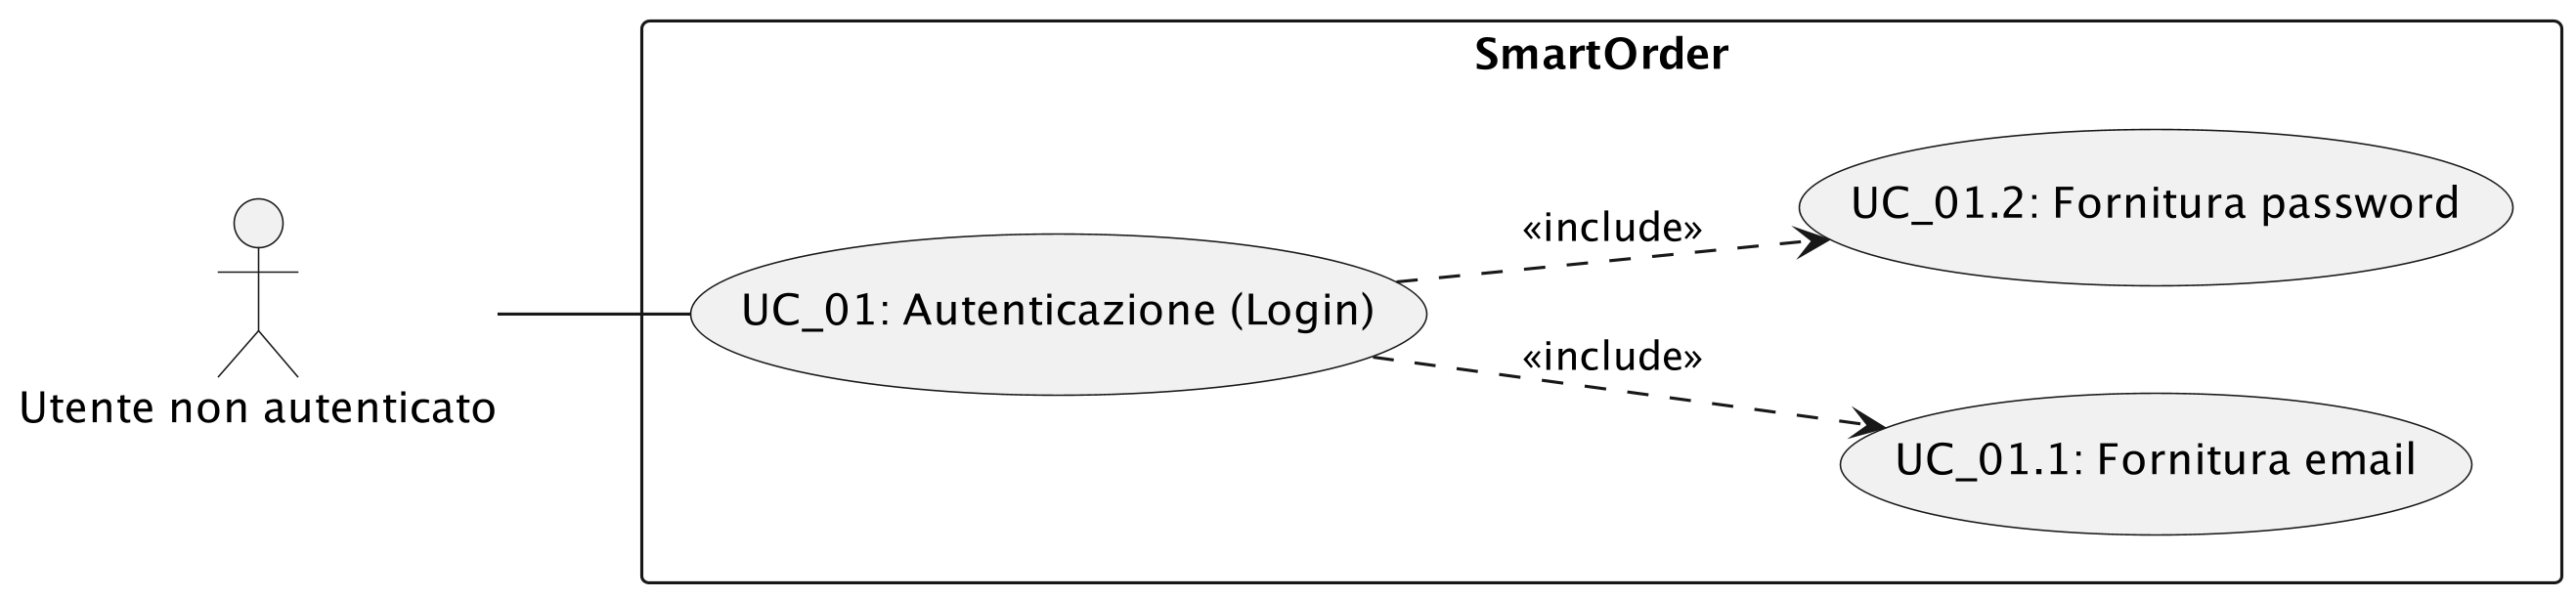
\includegraphics[width=0.8\textwidth]{uc-1.png}
    \caption{UC\_01: Autenticazione (Login)}
\end{figure}

\begin{itemize}
    \item \textbf{Attore\textsubscript{\textsc{g}} Principale}: Utente non autenticato
    \item \textbf{User Story}: Come Utente non autenticato, voglio accedere al sistema fornendo le mie credenziali, affinché io possa utilizzare la piattaforma nel mio ruolo specifico.
    \item \textbf{Scenario Principale}: 
    \begin{enumerate}
        \item Fornitura dell'email $\rightarrow$ Vedi \hyperref[uc_01.1]{UC\_01.1}
        \item Fornitura della password $\rightarrow$ Vedi \hyperref[uc_01.2]{UC\_01.2}
    \end{enumerate}
    \item \textbf{Precondizioni}:
    \begin{itemize}
        \item Il sistema è operativo.
        \item L'Utente non è autenticato ed è in fase di identificazione.
    \end{itemize}
    \item \textbf{Postcondizioni}:
    \begin{itemize}
        \item L'Utente viene autenticato e il sistema gli concede l'accesso all'area operativa corrispondente al proprio ruolo (Cliente o Operatore).
    \end{itemize}
    \item \textbf{Inclusioni}:
    \begin{itemize}
        \item \hyperref[uc_01.1]{UC\_01.1}, \hyperref[uc_01.2]{UC\_01.2}
    \end{itemize}
    \item \textbf{Estensioni}: Se il sistema rileva anomalie durante la fase di autenticazione come email o password non presenti, email o password errate, il sistema invia l'errore "Credenziali non valide" e non concede l'accesso.
    \item \textbf{Trigger}: L'Utente manifesta l'intenzione di accedere a una risorsa privata del sistema.
\end{itemize}

\subsubsection{UC\_01.1: Fornitura email}
\label{uc_01.1}
\begin{itemize}
    \item \textbf{Attore Principale}: Utente non autenticato
    \item \textbf{Scenario Principale}: L'Utente immette a sistema l'indirizzo email associato al proprio account.
    \item \textbf{Precondizioni}: Il sistema è in attesa di ricevere le credenziali.
    \item \textbf{Postcondizioni}: Il dato relativo all'email viene acquisito dal modulo d'accesso.
\end{itemize}

\subsubsection{UC\_01.2: Fornitura password}
\label{uc_01.2}
\begin{itemize}
    \item \textbf{Attore Principale}: Utente non autenticato
    \item \textbf{Scenario Principale}: L'Utente immette la propria password a sistema (con input visivamente offuscato per sicurezza).
    \item \textbf{Postcondizioni}: Il dato relativo alla password viene acquisito in modo protetto.
\end{itemize}

% -------------------------------------------------------------------

\subsection{UC\_02: Recupero password dimenticata}
\label{uc_02}

\begin{figure}[H]
    \centering 
    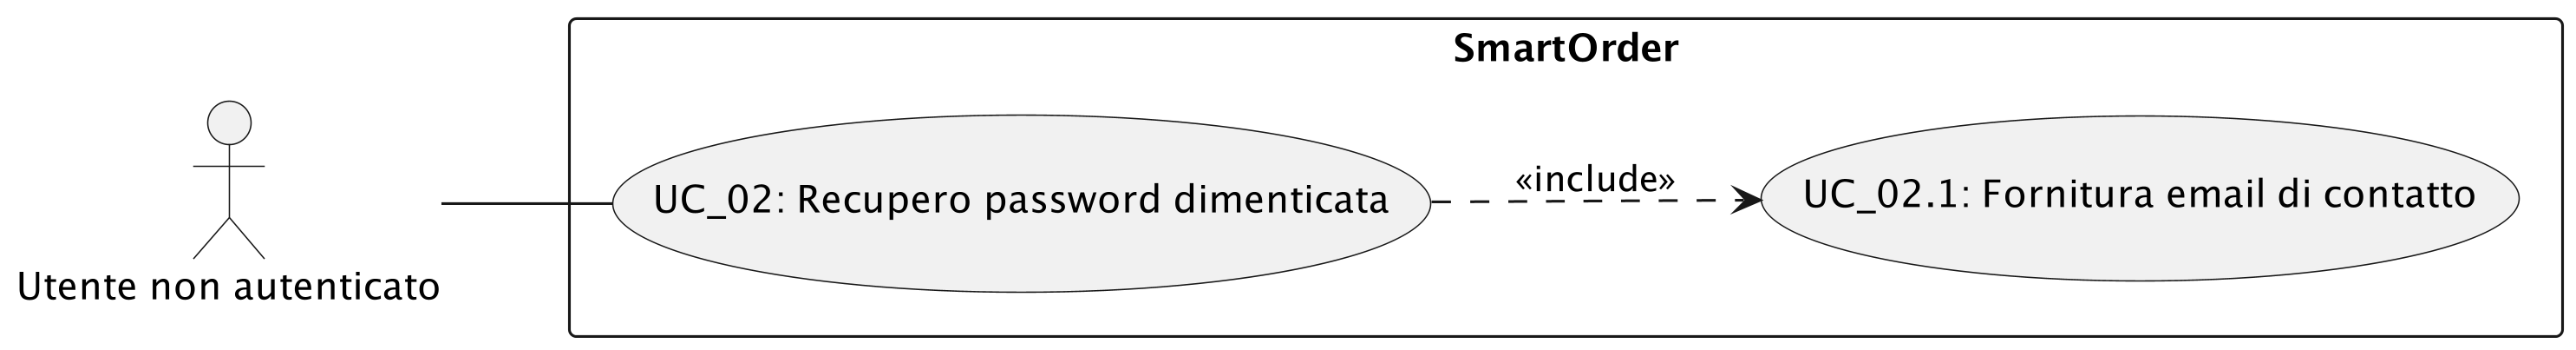
\includegraphics[width=0.8\textwidth]{uc-2.png}
    \caption{UC\_02: Recupero password dimenticata}
\end{figure}

\begin{itemize}
    \item \textbf{Attore Principale}: Utente non autenticato
    \item \textbf{User Story}: Come Utente non autenticato, voglio richiedere un link di ripristino per la mia password in caso di smarrimento.
    \item \textbf{Scenario Principale}:
    \begin{enumerate}
        \item L'Utente richiede l'accesso alla procedura di recupero.
        \item Fornitura dell'email di contatto $\rightarrow$ Vedi \hyperref[uc_02.1]{UC\_02.1}
    \end{enumerate}
    \item \textbf{Precondizioni}: L'Utente non è autenticato.
    \item \textbf{Postcondizioni}: Il sistema elabora la richiesta e predispone l'invio della comunicazione di ripristino.
    \item \textbf{Inclusioni}: \hyperref[uc_02.1]{UC\_02.1}
    \item \textbf{Trigger}: L'Utente manifesta la necessità di resettare le proprie credenziali tramite l'apposito comando.
\end{itemize}

\subsubsection{UC\_02.1: Fornitura email di contatto}
\label{uc_02.1}
\begin{itemize}
    \item \textbf{Attore Principale}: Utente non autenticato
    \item \textbf{Scenario Principale}: L'Utente immette a sistema il proprio indirizzo di posta elettronica all'interno del modulo dedicato.
\end{itemize}

% -------------------------------------------------------------------

\subsection{UC\_03: Terminazione Sessione (Logout)}
\label{uc_03}

\begin{figure}[H]
    \centering 
    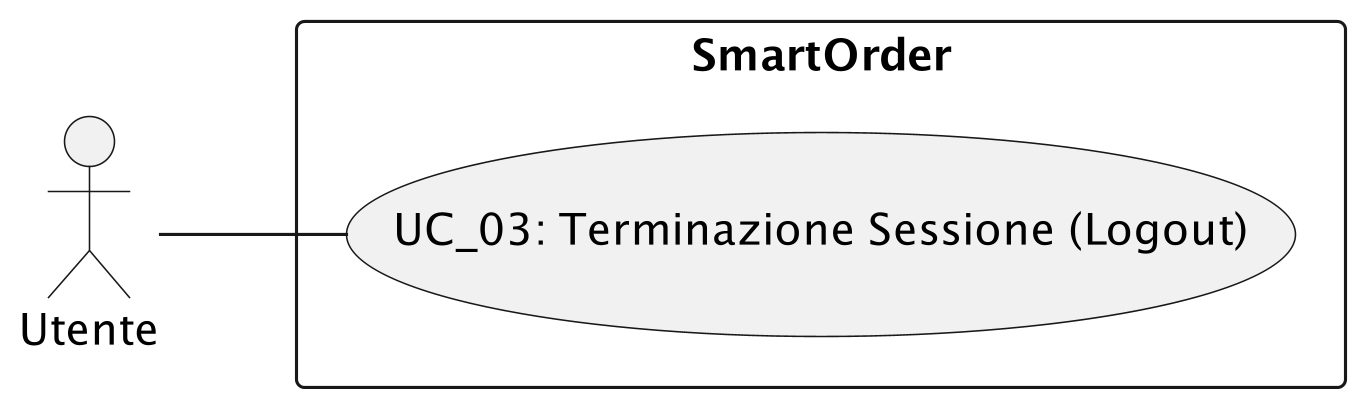
\includegraphics[width=0.8\textwidth]{uc-3.png}
    \caption{UC\_03: Terminazione Sessione (Logout)}
\end{figure}

\begin{itemize}
    \item \textbf{Attore Principale}: Utente
    \item \textbf{User Story}: Come Utente loggato, voglio poter terminare la mia sessione in totale sicurezza per prevenire accessi non autorizzati.
    \item \textbf{Scenario Principale}: L'Utente comanda l'uscita esplicita dal sistema interagendo con il controllo dedicato.
    \item \textbf{Precondizioni}: L'Utente possiede una sessione di autenticazione attiva.
    \item \textbf{Postcondizioni}: Il sistema invalida e distrugge la sessione corrente lato server, revocando le autorizzazioni dell'Utente e riportandolo alla schermata pubblica di login.
\end{itemize}

% -------------------------------------------------------------------

\subsection{UC\_04: Consultazione Area Personale}
\label{uc_04}

\begin{figure}[H]
    \centering 
    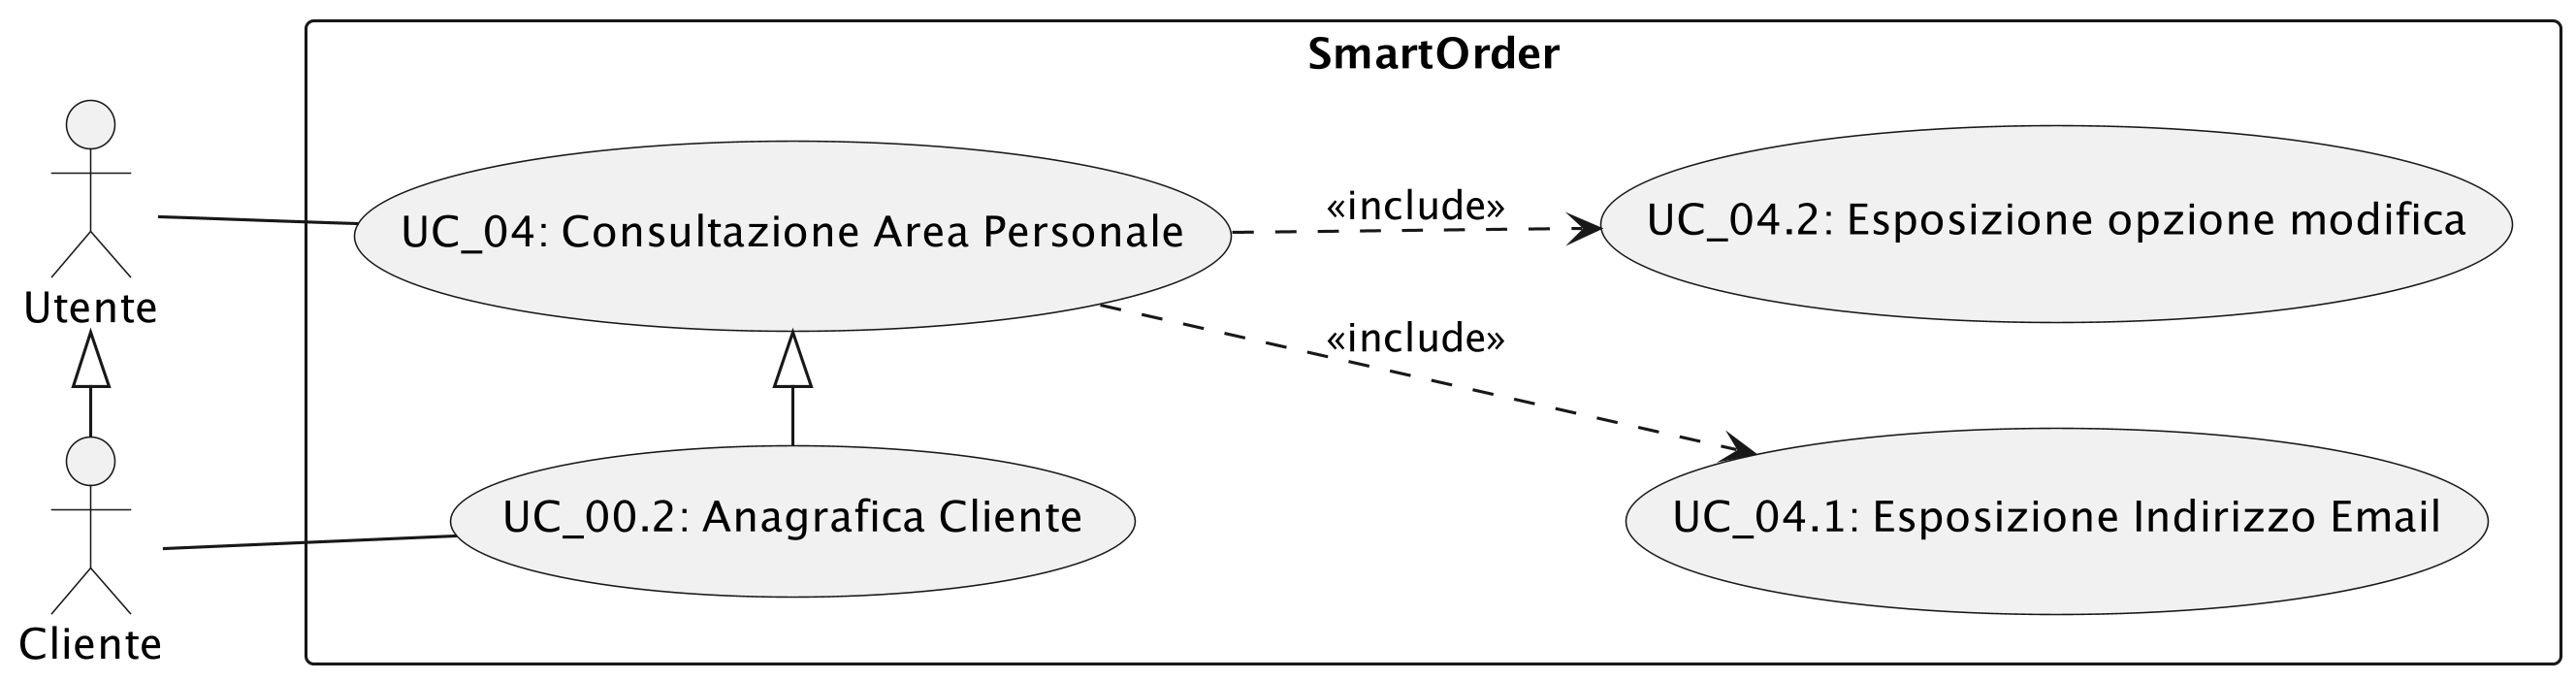
\includegraphics[width=0.8\textwidth]{uc-4.png}
    \caption{UC\_04: Consultazione Area Personale}
\end{figure}

\begin{itemize}
    \item \textbf{Attore Principale}: Utente
    \item \textbf{User Story}: Come Utente loggato, voglio accedere al riepilogo del mio profilo per verificare i dati anagrafici a me associati.
    \item \textbf{Scenario Principale}:
    \begin{enumerate}
        \item L'Utente richiede l'accesso alla rotta dedicata al profilo.
        \item \textit{[Solo se l'Utente possiede il ruolo "Cliente"]} Il sistema espone le informazioni anagrafiche aziendali $\rightarrow$ \hyperref[uc_00.2]{UC\_00.2}
        \item Esposizione dell'Indirizzo Email $\rightarrow$ Vedi \hyperref[uc_04.1]{UC\_04.1}
        \item Esposizione opzione di modifica credenziali $\rightarrow$ Vedi \hyperref[uc_04.2]{UC\_04.2}
    \end{enumerate}
    \item \textbf{Precondizioni}: L'Utente è riconosciuto dal sistema tramite sessione attiva.
    \item \textbf{Postcondizioni}: Il sistema rende disponibili i dati in base ai permessi di ruolo.
    \item \textbf{Inclusioni}: \hyperref[uc_00.2]{UC\_00.2}, \hyperref[uc_04.1]{UC\_04.1}, \hyperref[uc_04.2]{UC\_04.2}
    \item \textbf{Trigger}: Navigazione volontaria verso la sezione del profilo personale.
\end{itemize}

\subsubsection{UC\_04.1: Esposizione Indirizzo Email (Sola lettura)}
\label{uc_04.1}
\begin{itemize}
    \item \textbf{Attore Principale}: Utente
    \item \textbf{Scenario Principale}: Il sistema preleva dal DB locale e restituisce a schermo l'indirizzo email identificativo dell'Utente in modalità immutabile.
\end{itemize}

\subsubsection{UC\_04.2: Esposizione opzione di modifica credenziali}
\label{uc_04.2}
\begin{itemize}
    \item \textbf{Attore Principale}: Utente
    \item \textbf{Scenario Principale}: Il sistema presenta all'Utente l'accesso logico (es. pulsante o link) per avviare la mutazione della chiave di sicurezza, ponendosi in ascolto per l'attivazione del caso d'uso \hyperref[uc_05]{UC\_05}.
\end{itemize}

% -------------------------------------------------------------------

\subsection{UC\_05: Cambio Password}
\label{uc_05}

\begin{figure}[H]
    \centering 
    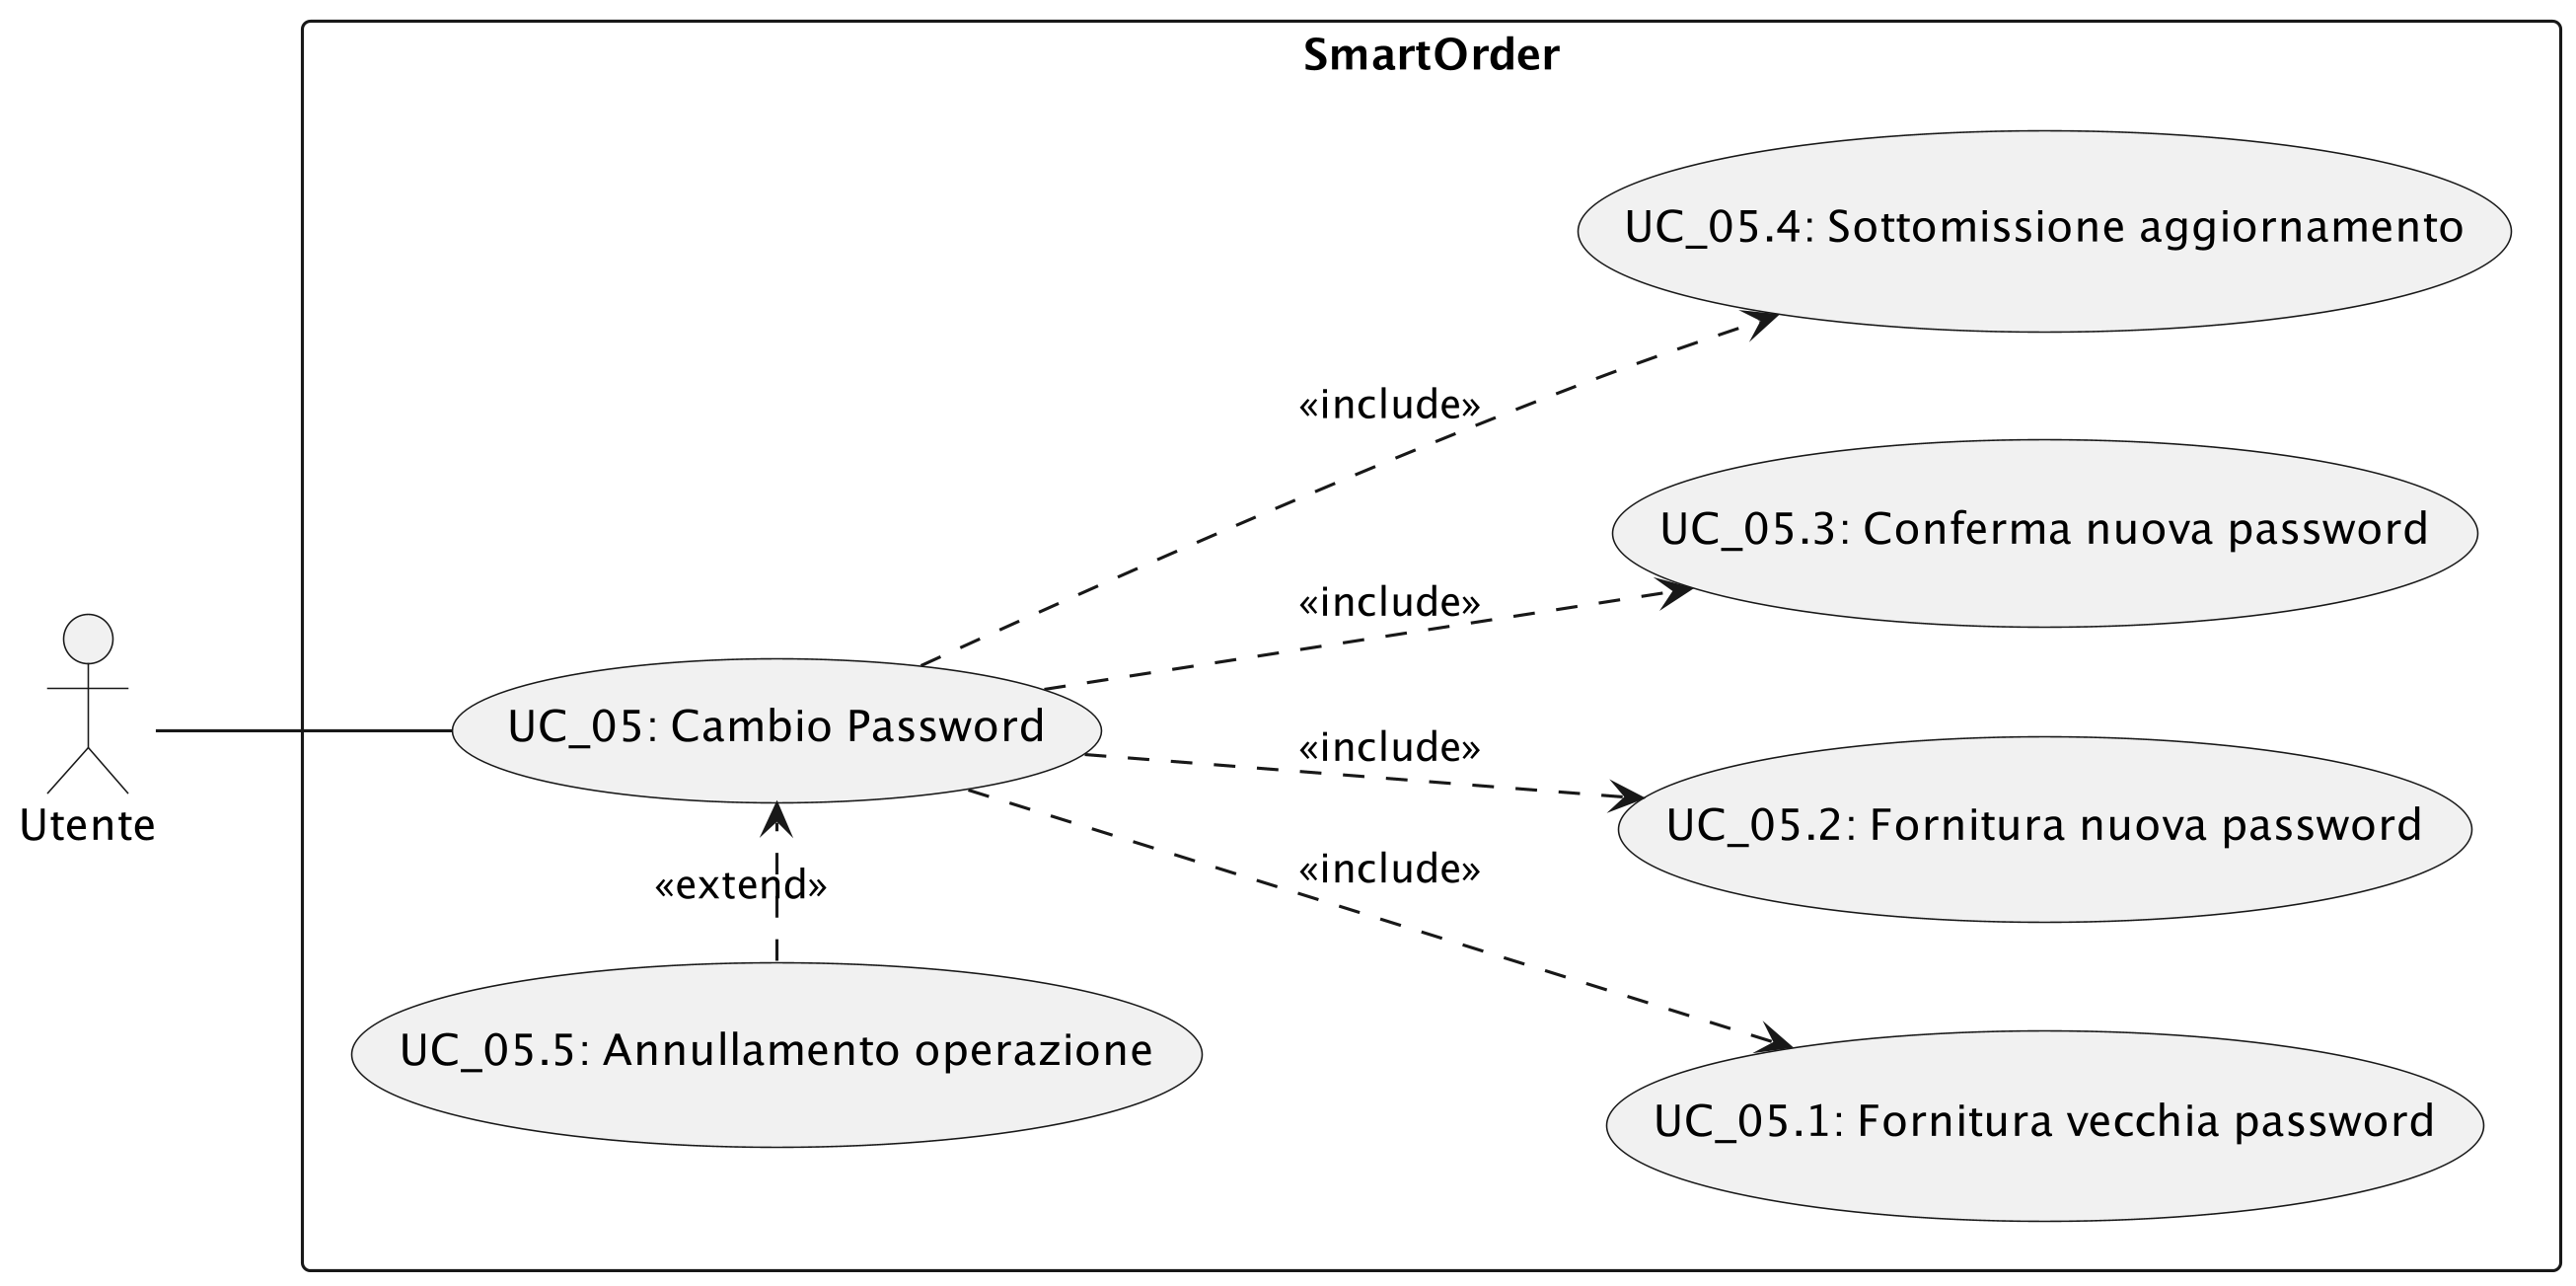
\includegraphics[width=0.8\textwidth]{uc-5.png}
    \caption{UC\_05: Cambio Password}
\end{figure}

\begin{itemize}
    \item \textbf{Attore Principale}: Utente
    \item \textbf{User Story}: Come Utente loggato, voglio rimpiazzare la mia password attuale con una nuova per garantire la sicurezza del mio account.
    \item \textbf{Nota Requisito}: Funzionalità classificata come requisito desiderabile.
    \item \textbf{Scenario Principale}:
    \begin{enumerate}
        \item Fornitura vecchia password $\rightarrow$ Vedi \hyperref[uc_05.1]{UC\_05.1}
        \item Fornitura nuova password $\rightarrow$ Vedi \hyperref[uc_05.2]{UC\_05.2}
        \item Fornitura conferma nuova password $\rightarrow$ Vedi \hyperref[uc_05.3]{UC\_05.3}
        \item Sottomissione aggiornamento $\rightarrow$ Vedi \hyperref[uc_05.4]{UC\_05.4}
    \end{enumerate}
    \item \textbf{Precondizioni}: L'Utente ha richiesto esplicitamente l'avvio della procedura dalla propria Area Personale.
    \item \textbf{Postcondizioni}: La sequenza di accesso crittografica dell'Utente viene aggiornata in via definitiva nel sistema.
    \item \textbf{Inclusioni}: \hyperref[uc_05.1]{UC\_05.1}, \hyperref[uc_05.2]{UC\_05.2}, \hyperref[uc_05.3]{UC\_05.3}, \hyperref[uc_05.4]{UC\_05.4}
    \item \textbf{Estensioni}: L'Utente opta per l'annullamento volontario dismettendo la procedura $\rightarrow$ Vedi \hyperref[uc_05.5]{UC\_05.5}
\end{itemize}

\subsubsection{UC\_05.1: Fornitura vecchia password}
\label{uc_05.1}
\begin{itemize}
    \item \textbf{Attore Principale}: Utente
    \item \textbf{Scenario Principale}: L'Utente immette a sistema la sequenza di sicurezza attualmente in vigore per scopi di convalida.
    \item \textbf{Estensioni}: Il sistema rileva che la sequenza corrente fornita non combacia con l'hash a database. L'operazione viene interrotta e viene generata un'anomalia.
\end{itemize}

\subsubsection{UC\_05.2: Fornitura nuova password}
\label{uc_05.2}
\begin{itemize}
    \item \textbf{Attore Principale}: Utente
    \item \textbf{Scenario Principale}: L'Utente immette a sistema la nuova sequenza desiderata, ottemperando alle policy architetturali di robustezza.
\end{itemize}

\subsubsection{UC\_05.3: Fornitura conferma nuova password}
\label{uc_05.3}
\begin{itemize}
    \item \textbf{Attore Principale}: Utente
    \item \textbf{Scenario Principale}: L'Utente re-immette la nuova sequenza per verificarne l'esattezza digitativa.
    \item \textbf{Estensioni}: Il sistema valuta l'assenza di identità tra la stringa di nuova password e quella di conferma. L'aggiornamento viene impedito con notifica d'errore.
\end{itemize}

\subsubsection{UC\_05.4: Sottomissione aggiornamento}
\label{uc_05.4}
\begin{itemize}
    \item \textbf{Attore Principale}: Utente
    \item \textbf{Scenario Principale}: L'Utente comanda il consolidamento delle modifiche. Il sistema esegue i controlli di validità e sovrascrive l'hash crittografico.
    \item \textbf{Postcondizioni}: La procedura si chiude restituendo una conferma di avvenuta esecuzione logica.
\end{itemize}

\subsubsection{UC\_05.5: Annullamento operazione}
\label{uc_05.5}
\begin{itemize}
    \item \textbf{Attore Principale}: Utente
    \item \textbf{Scenario Principale}: L'Utente comanda l'abbandono volontario della procedura.
    \item \textbf{Postcondizioni}: L'operazione decade transitoriamente. Il sistema dismette i parametri acquisiti ripristinando il normale stato di consultazione del profilo.
\end{itemize}

% -------------------------------------------------------------------
  
\subsection{UC\_06: Richiesta di contatto supporto tecnico}
\label{uc_06}

\begin{figure}[H]
    \centering 
    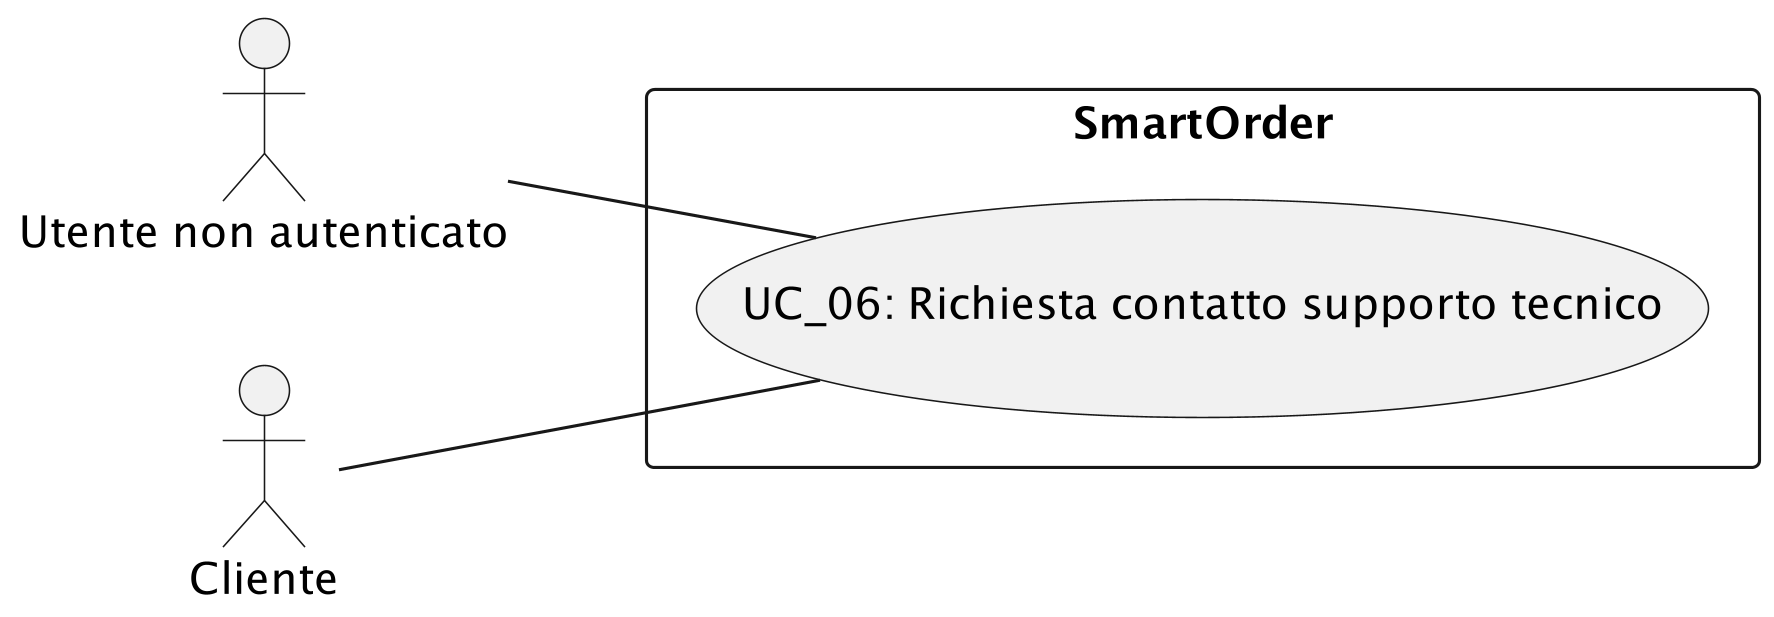
\includegraphics[width=0.8\textwidth]{uc-6.png}
    \caption{UC\_06: Richiesta di contatto supporto tecnico}
\end{figure}
 
\begin{itemize}
    \item \textbf{Attori}: Cliente, Utente non autenticato.
    \item \textbf{User Story}: Come cliente o utente non autenticato voglio avere un'opzione rapida per inoltrare comunicazioni amministrative tramite il mio sistema di posta elettronica nativo.
    \item \textbf{Scenario Principale}:
    \begin{enumerate}
        \item L'Utente comanda l'attivazione della funzionalità di contatto globale.
        \item Il sistema invoca il protocollo operativo standard (URI di tipo \textit{mailto:}).
        \item Il sistema operativo locale intercetta l'invocazione lanciando il software di composizione email, valorizzando automaticamente il destinatario.
        \item Il sistema imposta automaticamente l'email aziendale di supporto come destinatario predefinito.
        \item Il controllo del flusso esce dal dominio applicativo della webapp. L'utente completa la stesura dell'email tramite il proprio client esterno (compilando l'oggetto, il corpo del testo ed eventualmente definendo il mittente) e ne finalizza l'invio in totale autonomia.
    \end{enumerate}
    \item \textbf{Precondizioni}: Il cliente ha accesso alle funzionalità generali dell'applicativo. L'utente non registrato ha accesso alla pagina di login. Il dispositivo locale possiede un client email configurato.
    \item \textbf{Postcondizioni}: L'azione esce dal perimetro dell'applicativo web.
    \item \textbf{Trigger}: Manifestazione della necessità di instaurare un dialogo extra-sistema.
\end{itemize}

% ==========================================
% GRUPPO B: INTERAZIONE CHAT E AI
% ==========================================

\subsection{UC\_07: Consultazione Chat (Live)}
\label{uc_07}

\begin{figure}[H]
    \centering 
    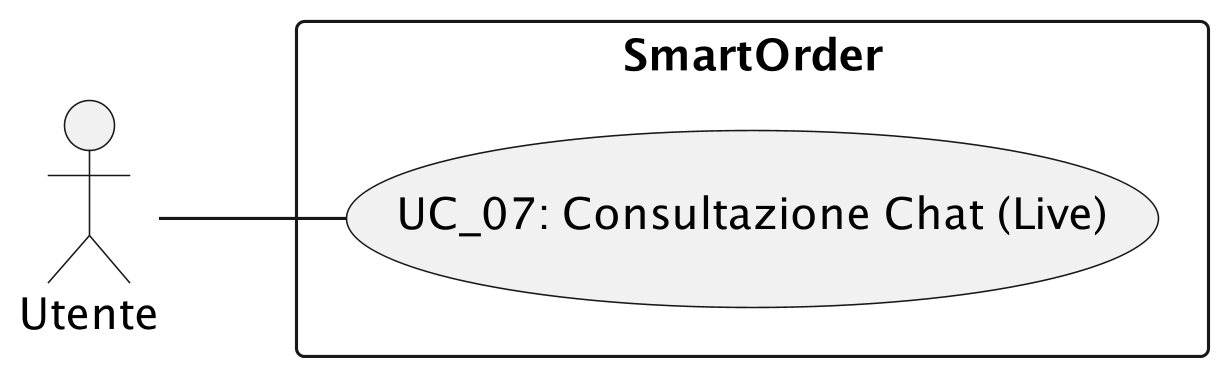
\includegraphics[width=0.8\textwidth]{uc-7.png}
    \caption{UC\_07: Consultazione Chat}
\end{figure}

\begin{itemize}
    \item \textbf{Attore Principale}: Utente
    \item \textbf{User Story}: Come Utente loggato (Cliente nel front-end o Operatore nel backoffice), voglio poter consultare lo storico live dei messaggi di una sessione, per avere chiara l'evoluzione della conversazione e il contesto delle richieste.
    \item \textbf{Scenario Principale}: 
    \begin{enumerate}
        \item L'Utente accede all'interfaccia della sessione di chat (il Cliente alla propria, l'Operatore tramite la scheda di assistenza del ticket).
        \item Il sistema recupera dal database la lista di oggetti "Messaggio" associata alla sessione attiva.
        \item Il sistema itera sulla lista ed espone la cronologia a schermo, distinguendo visivamente l'autore di ogni singolo oggetto:
        \begin{itemize}
            \item \textit{Messaggi originati dal Cliente}: Esposti come input originario della richiesta.
            \item \textit{Messaggi originati dal Sistema/Supporto}: Esposti come risposte, aggregando in modo trasparente sia gli output generati automaticamente dal modello LLM, sia i messaggi manuali inseriti dall'Operatore in fase di subentro (Human Handoff).
        \end{itemize}
        \item Il sistema si pone in ascolto asincrono per l'aggiornamento della lista in tempo reale.
    \end{enumerate}
    \item \textbf{Precondizioni}: L'Utente ha i permessi per visualizzare la sessione.
    \item \textbf{Postcondizioni}: La vista renderizza lo storico e si aggiorna dinamicamente aggiungendo nuovi oggetti "Messaggio" alla lista esposta.
    \item \textbf{Trigger}: Caricamento dell'interfaccia della chat o ricezione di un nuovo pacchetto dati.
\end{itemize}

% -------------------------------------------------------------------

\subsection{UC\_08: Sottomissione Input Multimodale}
\label{uc_08}

\begin{figure}[H]
    \centering 
    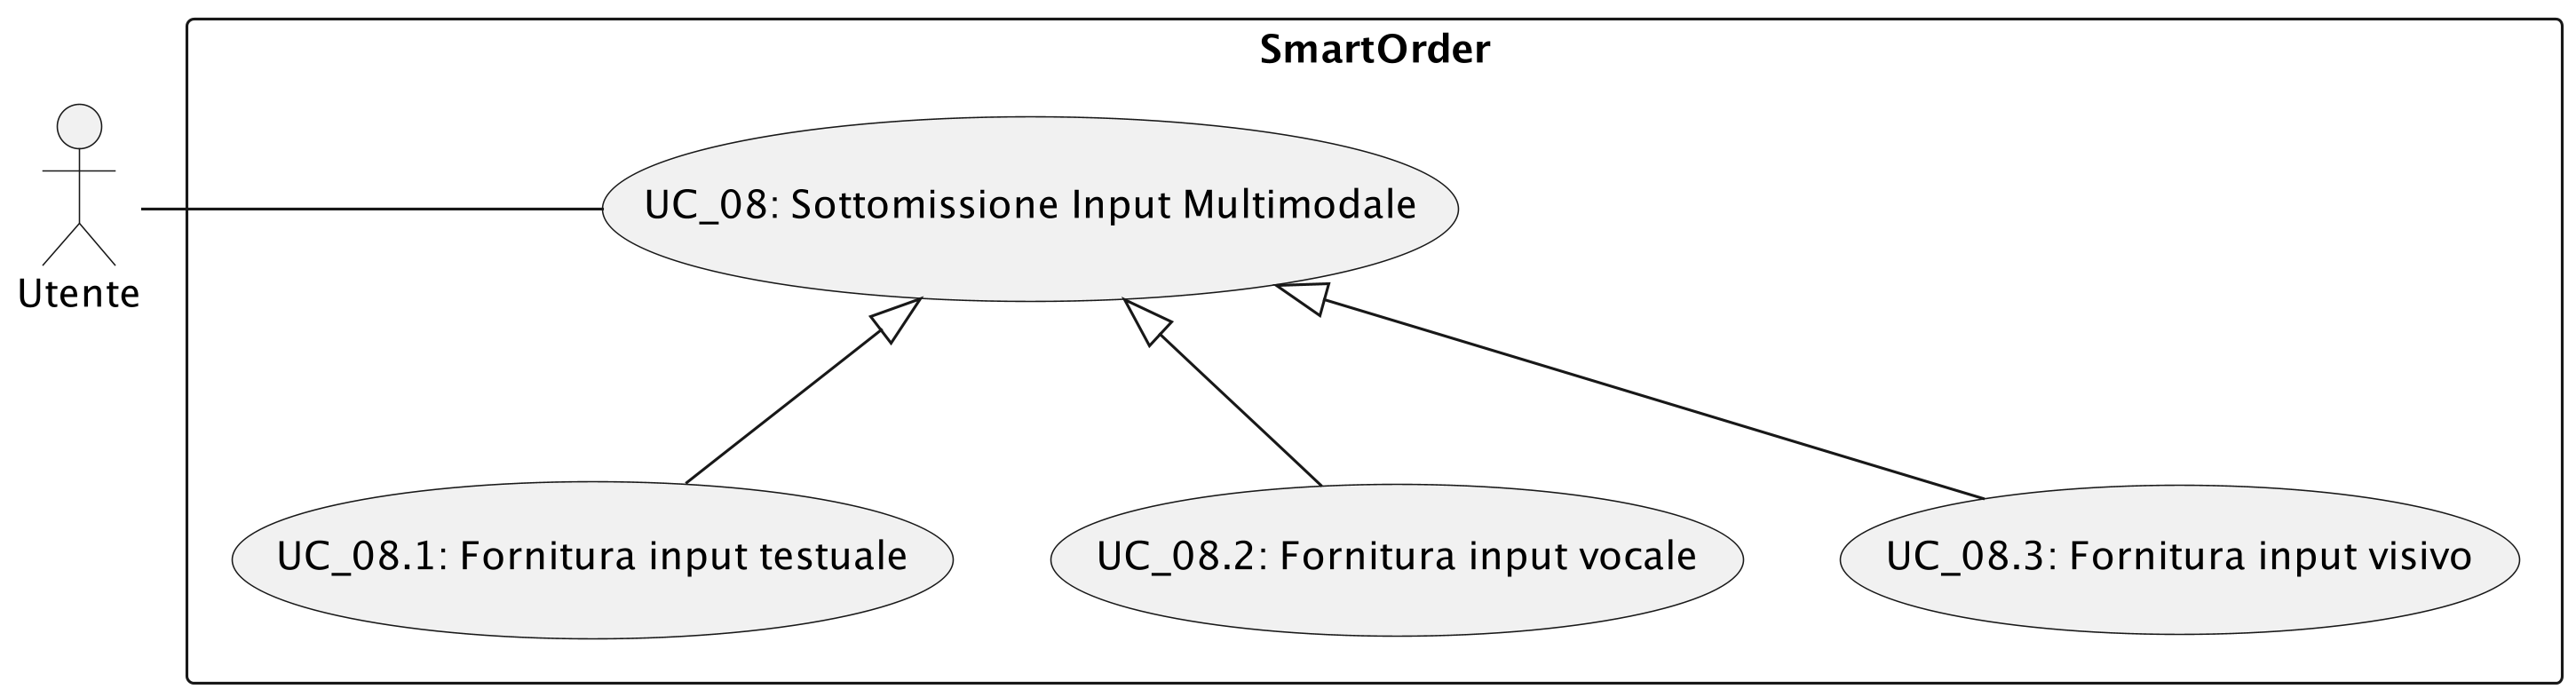
\includegraphics[width=0.8\textwidth]{uc-8.png}
    \caption{UC\_08: Sottomissione Input Multimodale}
\end{figure}

\begin{itemize}
    \item \textbf{Attore Principale}: Utente
    \item \textbf{User Story}: Come Utente, voglio poter inviare richieste al sistema utilizzando diverse modalità (testo, voce, immagini) per formulare un comando nel modo più efficiente possibile a seconda del mio contesto.
    \item \textbf{Scenario Principale}:
    \begin{enumerate}
        \item L'Utente determina la modalità di inserimento dati preferita interagendo con l'interfaccia.
        \item Immissione tramite canale testuale $\rightarrow$ Vedi \hyperref[uc_08.1]{UC\_08.1}
        \item Immissione tramite canale vocale $\rightarrow$ Vedi \hyperref[uc_08.2]{UC\_08.2}
        \item Immissione tramite acquisizione visiva $\rightarrow$ Vedi \hyperref[uc_08.3]{UC\_08.3}
    \end{enumerate}
    \item \textbf{Precondizioni}:
    \begin{itemize}
        \item L'Utente ha accesso ai controlli di interazione della conversazione attiva.
    \end{itemize}
    \item \textbf{Postcondizioni}:
    \begin{itemize}
        \item Il payload (testuale o multimediale) viene confezionato dal frontend e trasmesso al backend locale per il processamento o l'inoltro all'Intelligenza Artificiale. Il sistema si pone in attesa asincrona della risposta.
    \end{itemize}
    \item \textbf{Specializzazioni}:
    \begin{itemize}
        \item \hyperref[uc_08.1]{UC\_08.1}, \hyperref[uc_08.2]{UC\_08.2}, \hyperref[uc_08.3]{UC\_08.3}
    \end{itemize}
    \item \textbf{Trigger}: L'Utente avvia la composizione di un nuovo messaggio.
\end{itemize}

\subsubsection{UC\_08.1: Fornitura di input testuale}
\label{uc_08.1}
\begin{itemize}
    \item \textbf{Attore Principale}: Utente
    \item \textbf{Scenario Principale}: L'Utente formula il proprio messaggio digitandolo nel modulo dedicato e ne comanda l'invio logico.
    \item \textbf{Postcondizioni}: La stringa testuale viene validata e immessa nel flusso dati verso l'analizzatore semantico.
    \item \textbf{Estensioni}:
    \begin{itemize}
        \item Se l'input testuale eccede i limiti dimensionali architetturali $\rightarrow$ Il sistema interrompe l'invio preventivamente, mantiene il testo a disposizione per correzioni e notifica l'impossibilità di procedere a causa dell'eccessiva lunghezza.
    \end{itemize}
\end{itemize}

\subsubsection{UC\_08.2: Fornitura di input vocale}
\label{uc_08.2}
\begin{itemize}
    \item \textbf{Attore Principale}: Utente
    \item \textbf{Scenario Principale}: L'Utente avvia l'acquisizione microfonica, detta la richiesta vocalmente e arresta la registrazione comandandone la trasmissione.
    \item \textbf{Precondizioni}: Il dispositivo ospite possiede i permessi hardware di cattura audio.
    \item \textbf{Postcondizioni}: Il file audio viene trasmesso al modulo Speech-to-Text per la conversione in stringa elaborabile.
    \item \textbf{Estensioni}:
    \begin{itemize}
        \item Se il file audio eccede il peso massimo consentito (es. 10MB) $\rightarrow$ Il caricamento viene inibito con esposizione di notifica d'errore.
    \end{itemize}
\end{itemize}

\subsubsection{UC\_08.3: Fornitura di input visivo (Immagine)}
\label{uc_08.3}
\begin{itemize}
    \item \textbf{Attore Principale}: Utente
    \item \textbf{Nota Requisito}: Questa funzionalità è classificata come requisito desiderabile.
    \item \textbf{Scenario Principale}: L'Utente innesca la funzione di caricamento media e seleziona la fonte di acquisizione (fotocamera hardware, galleria locale o file system).
    \item \textbf{Precondizioni}: L'ambiente operativo supporta i moduli di elaborazione OCR (Optical Character Recognition).
    \item \textbf{Postcondizioni}: L'immagine scelta viene immessa nella pipeline per l'estrazione logica del contenuto testuale o l'identificazione prodotto.
    \item \textbf{Estensioni}:
    \begin{itemize}
        \item Se l'immagine selezionata eccede il peso massimo (es. 5MB) $\rightarrow$ L'upload viene bloccato e il sistema notifica l'impossibilità di processare il file.
    \end{itemize}
\end{itemize}

% -------------------------------------------------------------------

\subsection{UC\_09: Feedback messaggi AI}
\label{uc_09}

\begin{figure}[H]
    \centering 
    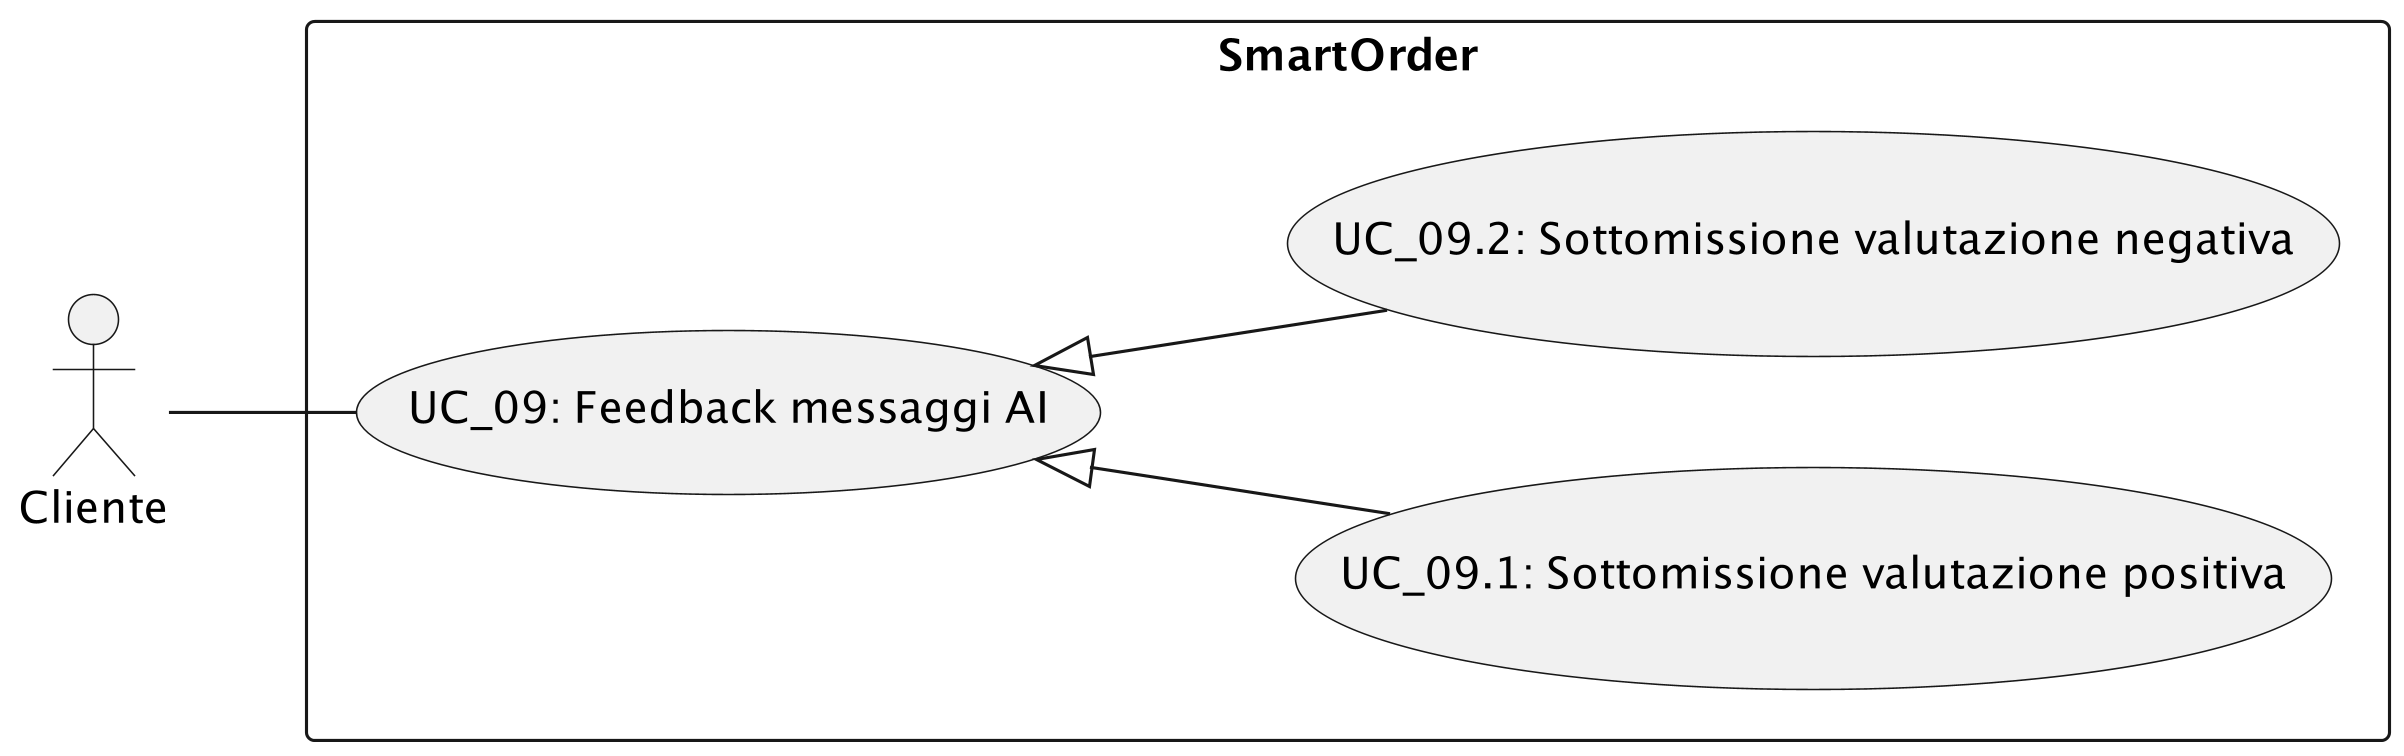
\includegraphics[width=0.8\textwidth]{uc-9.png}
    \caption{UC\_09: Classificazione e Feedback Risposta AI}
\end{figure}

\begin{itemize}
    \item \textbf{Attore Principale}: Cliente
    \item \textbf{User Story}: Come Cliente, voglio poter giudicare l'accuratezza semantica delle risposte del sistema per contribuire al perfezionamento dell'Intelligenza Artificiale aziendale.
    \item \textbf{Scenario Principale}:
    \begin{enumerate}
        \item Il Cliente valuta intellettualmente l'output generato dall'LLM.
        \item Sottomissione di giudizio positivo $\rightarrow$ Vedi \hyperref[uc_09.1]{UC\_09.1}
        \item Sottomissione di giudizio negativo e segnalazione anomalia $\rightarrow$ Vedi \hyperref[uc_09.2]{UC\_09.2}
    \end{enumerate}
    \item \textbf{Precondizioni}:
    \begin{itemize}
        \item Il sistema ha esposto almeno un output generato dal modello linguistico e i controlli di valutazione sono abilitati.
    \end{itemize}
    \item \textbf{Postcondizioni}:
    \begin{itemize}
        \item Il feedback viene registrato nel database locale e relazionato all'identificativo univoco della transazione AI (Log).
    \end{itemize}
    \item \textbf{Specializzazioni}:
    \begin{itemize}
        \item \hyperref[uc_09.1]{UC\_09.1}, \hyperref[uc_09.2]{UC\_09.2}
    \end{itemize}
    \item \textbf{Trigger}: Il Cliente matura un'opinione circa la congruità dell'output ricevuto.
\end{itemize}

\subsubsection{UC\_09.1: Sottomissione di valutazione positiva}
\label{uc_09.1}
\begin{itemize}
    \item \textbf{Attore Principale}: Cliente
    \item \textbf{Scenario Principale}: Il Cliente comanda l'assegnazione di un feedback logico positivo. Il sistema riceve l'impulso e lo archivia silenziamente.
    \item \textbf{Postcondizioni}: L'interfaccia inibisce valutazioni duplicate sul medesimo output.
\end{itemize}

\subsubsection{UC\_09.2: Sottomissione di valutazione negativa}
\label{uc_09.2}
\begin{itemize}
    \item \textbf{Attore Principale}: Cliente
    \item \textbf{Scenario Principale}:
    \begin{enumerate}
        \item Il Cliente manifesta l'intento di classificare la risposta come errata, causando l'esposizione di un modulo dedicato.
        \item Il Cliente seleziona obbligatoriamente i tag contestuali che definiscono la natura dell'errore (es. Errore semantico, Errore quantità).
        \item Il Cliente immette del testo libero opzionale per fornire note integrative.
        \item Il Cliente comanda il consolidamento e l'invio della segnalazione.
    \end{enumerate}
    \item \textbf{Postcondizioni}: Il sistema aggrega i parametri in un payload strutturato e genera un record d'errore (Stato "Da gestire") destinato all'ispezione nel backoffice.
    \item \textbf{Estensioni}:
    \begin{itemize}
        \item Abbandono volontario $\rightarrow$ Il Cliente comanda l'interruzione della stesura. Il modulo si chiude e i dati temporanei decadono.
    \end{itemize}
\end{itemize}

% -------------------------------------------------------------------

\subsection{UC\_10: Azzeramento del Contesto (Reset Sessione)}
\label{uc_10}

\begin{figure}[H]
    \centering 
    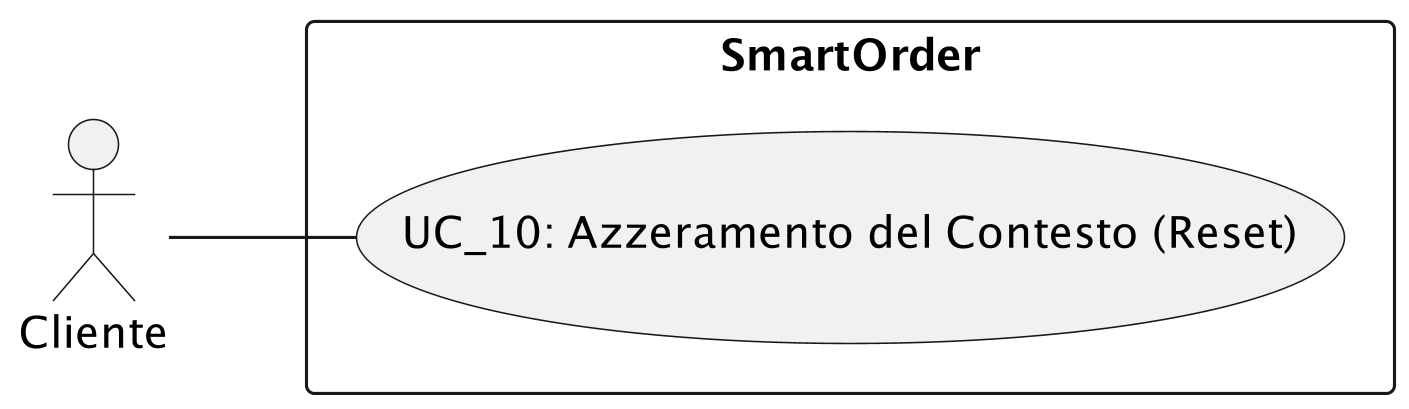
\includegraphics[width=0.8\textwidth]{uc-10.png}
    \caption{UC\_10: Azzeramento del Contesto (Reset Sessione)}
\end{figure}

\begin{itemize}
    \item \textbf{Attore Principale}: Cliente
    \item \textbf{User Story}: Come Cliente, voglio poter ripulire completamente la memoria dell'Intelligenza Artificiale per evitare interferenze tra il mio prossimo ordine e le richieste passate.
    \item \textbf{Scenario Principale}:
    \begin{enumerate}
        \item Il Cliente comanda l'instaurazione di una nuova sessione operativa tramite l'apposito controllo.
        \item Il sistema recepisce l'input ed esegue le procedure di bonifica logica lato server.
    \end{enumerate}
    \item \textbf{Precondizioni}:
    \begin{itemize}
        \item Non vi sono richieste di supporto tecnico (Ticket) pendenti o in lavorazione per la sessione attuale.
    \end{itemize}
    \item \textbf{Postcondizioni}:
    \begin{itemize}
        \item Il sistema rigetta il tracciato conversazionale precedente, svuota il carrello in memoria e associa il client a un nuovo Session ID vergine.
    \end{itemize}
    \item \textbf{Trigger}: Il Cliente necessita di un cambio radicale di contesto d'acquisto o desidera abortire la composizione in atto.
\end{itemize}

% ==========================================
% GRUPPO C: GESTIONE CARRELLO E RICERCA
% ==========================================

\subsection*{Ricerca e Aggiunta Manuale (UC\_11, UC\_12)}

\begin{figure}[H]
    \centering 
    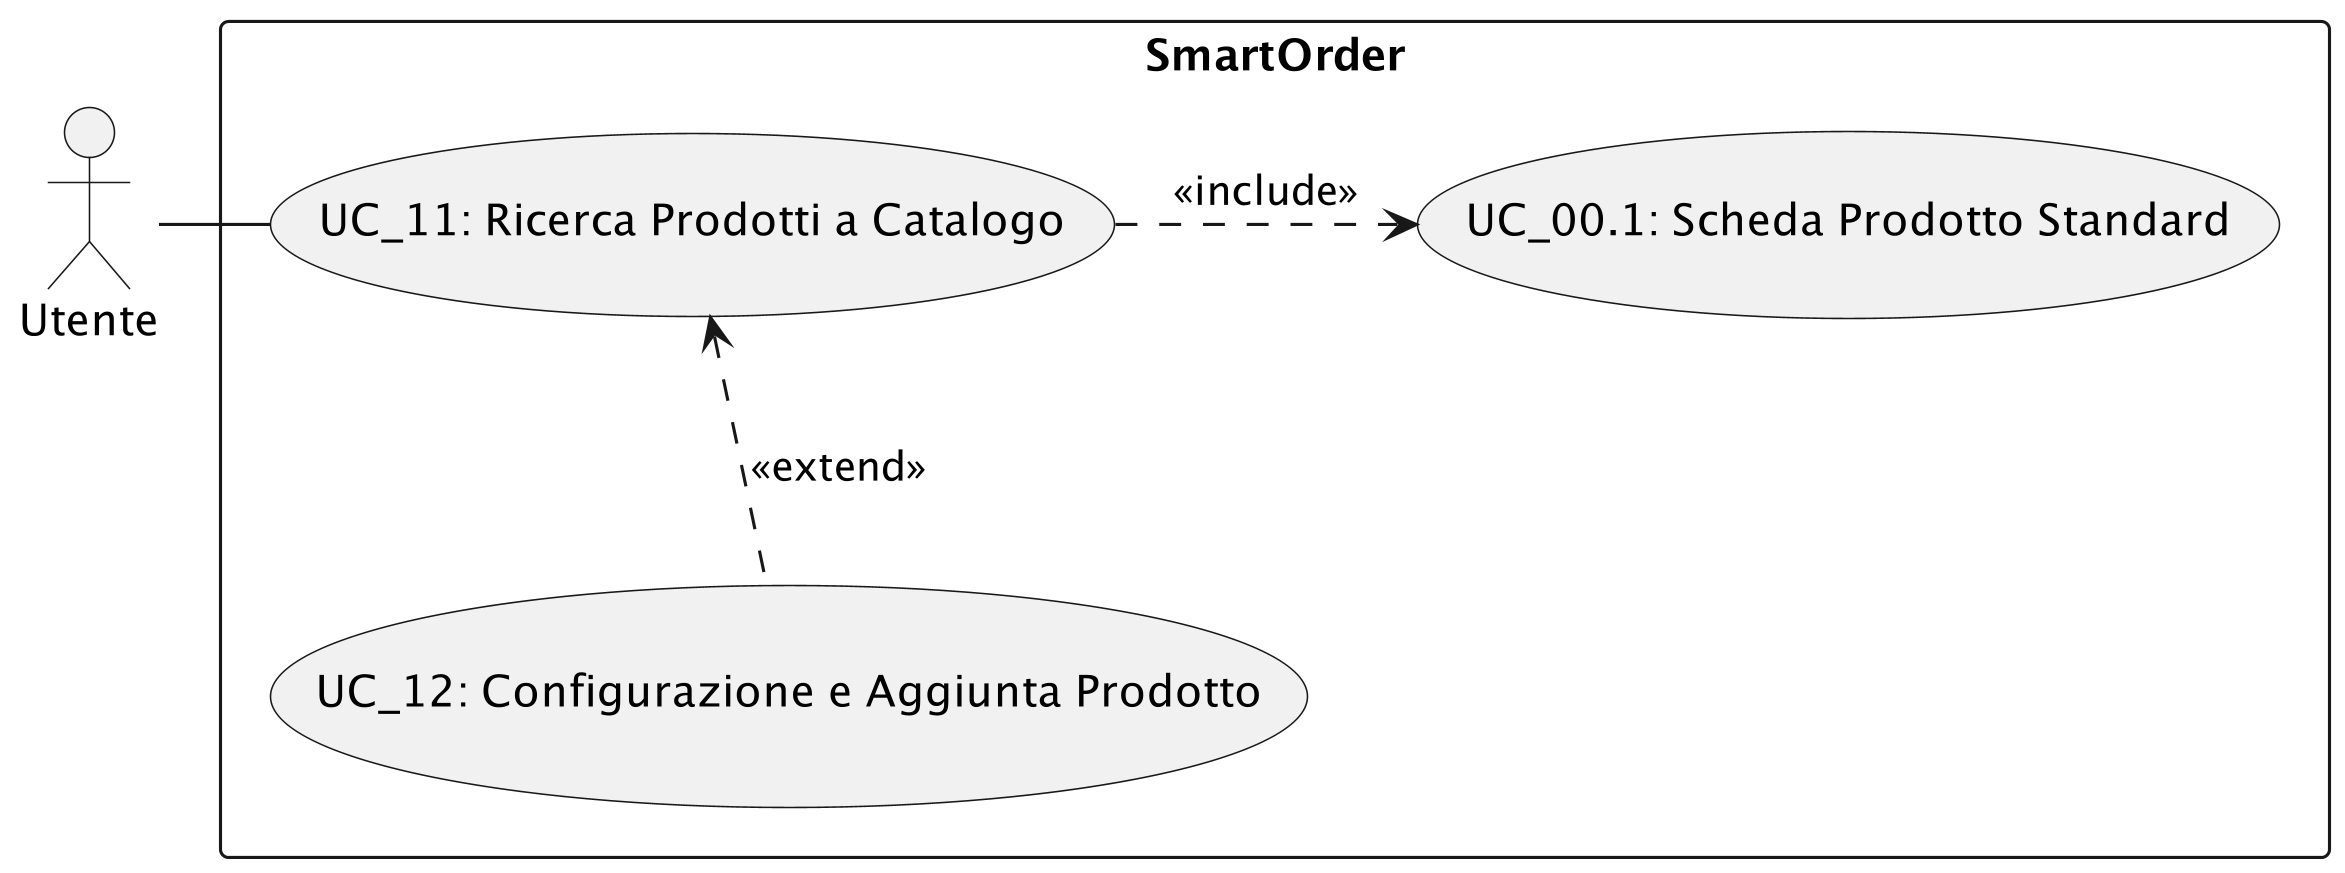
\includegraphics[width=0.8\textwidth]{uc-11.png}
    \caption{UC\_11, UC\_12: Ricerca e Aggiunta Manuale}
\end{figure}

\subsection{UC\_11: Ricerca Prodotti a Catalogo}
\label{uc_11}

\begin{itemize}
    \item \textbf{Attore Principale}: Utente
    \item \textbf{User Story}: Come Utente loggato (Cliente nel front-end o Operatore in assistenza), voglio poter cercare un prodotto specifico all'interno dell'assortimento tramite una query testuale, affinché io possa individuarlo e aggiungerlo all'ordine senza impiegare l'interazione conversazionale.
    \item \textbf{Parametri di Ricerca}: Il sistema confronta la stringa di ricerca con i seguenti attributi a database: \textit{Nome Prodotto}, \textit{Codice Articolo} (es. AC305) e \textit{Categoria/Sottocategoria} (es. ACQUE, PREMIUM).
    \item \textbf{Scenario Principale}: 
    \begin{enumerate}
        \item L'Utente immette una stringa di testo nel modulo di ricerca dedicato all'aggiunta articoli.
        \item Il sistema intercetta l'input e interroga dinamicamente il database locale filtrando i prodotti in base ai Parametri di Ricerca definiti.
        \item Il sistema genera e aggiorna a schermo una lista contestuale dei risultati (Live Search).
        \item Per ogni referenza individuata, il sistema espone il nome e i relativi metadati anagrafici e logistici $\rightarrow$ Include: \hyperref[uc_00.1]{UC\_00.1}.
    \end{enumerate}
    \item \textbf{Precondizioni}: L'interfaccia carrello è attiva (propria per il Cliente, in delega per l'Operatore). Il catalogo interrogabile è già stato pre-filtrato applicando le regole di visibilità e assortimento specifiche per il Cliente in gestione.
    \item \textbf{Postcondizioni}: L'elenco dei risultati pertinenti è visibile e interattivo, pronto per la selezione. Nessuna modifica viene apportata allo stato del carrello in questa fase.
    \item \textbf{Inclusioni}: \hyperref[uc_00.1]{UC\_00.1}
    \item \textbf{Trigger}: Immissione di caratteri nel campo di ricerca articoli.
\end{itemize}

% -------------------------------------------------------------------

\subsection{UC\_12: Configurazione e Aggiunta Prodotto al Carrello}
\label{uc_12}

\begin{itemize}
    \item \textbf{Attore Principale}: Utente
    \item \textbf{User Story}: Come Utente, una volta individuato l'articolo d'interesse, voglio poterne specificare la quantità desiderata, e confermarne l'inserimento nel carrello corrente.
    \item \textbf{Scenario Principale}: 
    \begin{enumerate}
        \item L'Utente seleziona un prodotto dalla lista dei risultati di ricerca.
        \item Il sistema espone i dettagli di configurazione per l'acquisto, indicando gli eventuali vincoli logistici (es. multipli di vendita o "Venduto in casse").
        \item L'Utente regola la quantità desiderata tramite incremento/decremento logico o immissione numerica diretta.
        \item L'Utente comanda l'inserimento definitivo tramite l'azione "Aggiungi al carrello".
        \item Il sistema valida la richiesta, registra l'articolo con la rispettiva quantità nel database di sessione associato al Cliente in gestione e aggiorna il contatore totale.
    \end{enumerate}
    \item \textbf{Precondizioni}: Il prodotto selezionato fa parte dell'assortimento visibile ed è correntemente disponibile a sistema.
    \item \textbf{Postcondizioni}: Lo stato del carrello viene mutato. L'articolo entra a far parte della lista degli elementi pronti per il checkout logico. Il modulo di configurazione viene chiuso.
    \item \textbf{Estensioni}:
    \begin{itemize}
        \item \textit{Violazione vincoli di quantità}: Se l'Utente tenta l'inserimento di un valore non consentito (es. valore nullo, negativo o non rispettoso dei multipli di cassa previsti), il sistema impedisce l'invio e applica una correzione forzata verso il limite o il multiplo accettabile più vicino.
        \item \textit{Annullamento dell'azione}: L'Utente dismette volontariamente la scheda di configurazione prima della conferma. Lo stato del carrello rimane inalterato.
    \end{itemize}
    \item \textbf{Trigger}: Selezione esplicita di una referenza dall'elenco.
\end{itemize}
% -------------------------------------------------------------------

\subsection*{Visualizzazione e Gestione Carrello (UC\_13, UC\_14)}

\begin{figure}[H]
    \centering 
    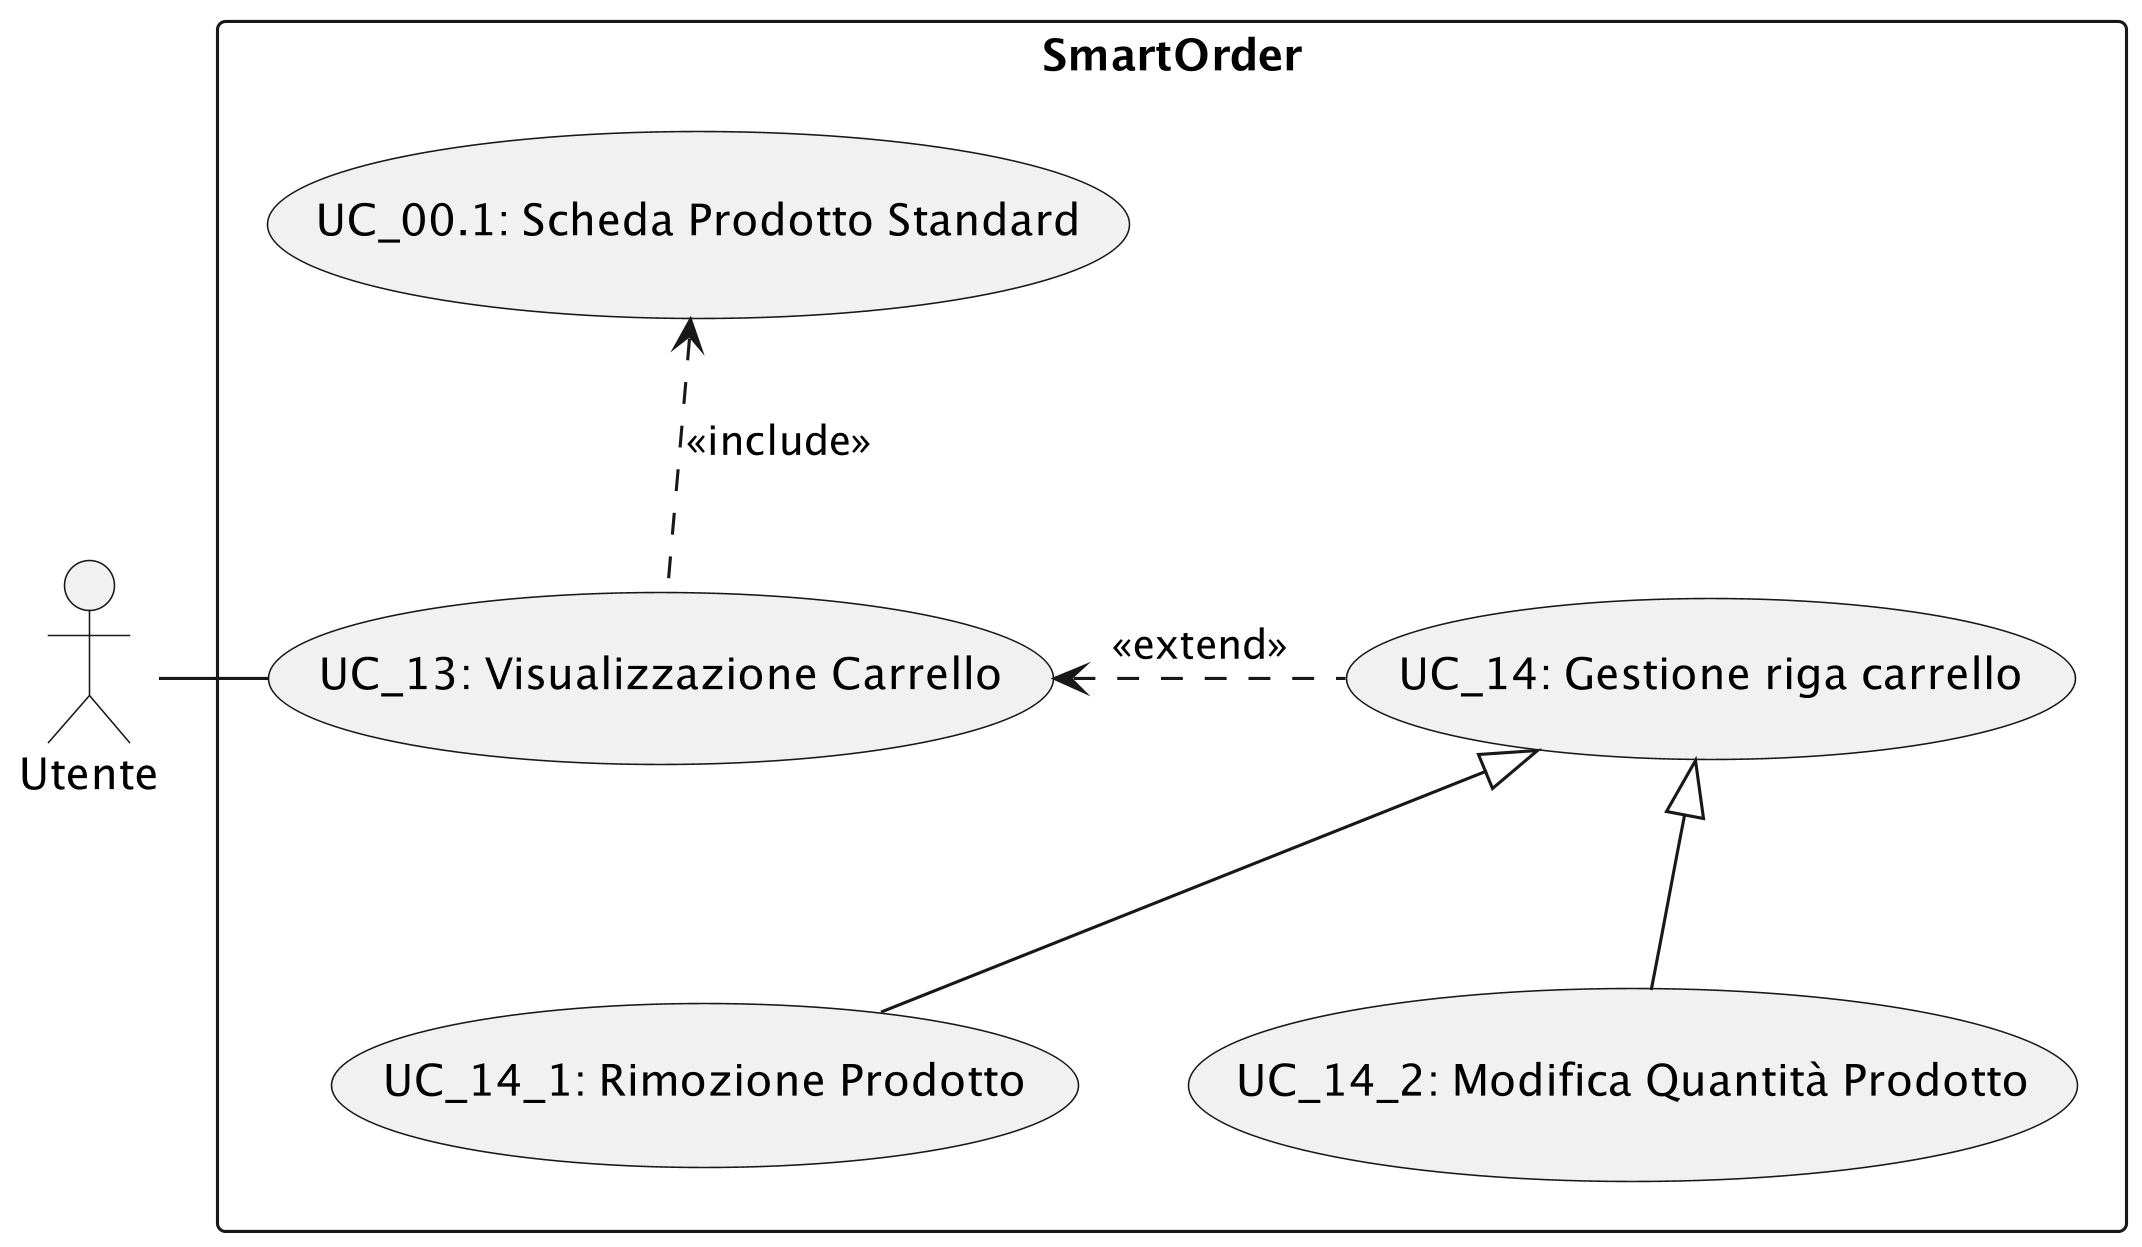
\includegraphics[width=0.8\textwidth]{uc-13.png}
    \caption{UC\_13, UC\_14: Visualizzazione e Gestione Carrello}
\end{figure}

\subsection{UC\_13: Visualizzazione Carrello}
\label{uc_13}

\begin{itemize}
    \item \textbf{Attore Principale}: Utente
    \item \textbf{User Story}: Come Utente loggato (Cliente nel front-end o Operatore in assistenza), voglio poter visualizzare l'elenco dei prodotti attualmente inseriti nel carrello per verificarne la correttezza logistica prima di procedere alla finalizzazione.
    \item \textbf{Scenario Principale}: 
    \begin{enumerate}
        \item L'Utente richiede l'accesso alla vista di riepilogo del carrello (il Cliente navigando alla pagina dedicata, l'Operatore accedendovi tramite la scheda del ticket di subentro).
        \item Il sistema interroga il database di sessione associato all'utenza in gestione.
        \item \textit{Caso A (Carrello Valorizzato)}: Il sistema itera sugli articoli presenti e renderizza una lista strutturata. Per ogni riga, espone l'origine d'inserimento (es. tramite un banner per le referenze aggiunte dall'AI), la quantità correntemente ordinata e i metadati logistici $\rightarrow$ Include: \hyperref[uc_00.1]{UC\_00.1}.
        \item \textit{Caso B (Carrello Vuoto)}: Il sistema rileva l'assenza di referenze e renderizza un layout testuale di avviso, inibendo visivamente i controlli di checkout.
    \end{enumerate}
    \item \textbf{Precondizioni}: L'Utente ha i permessi operativi sulla sessione corrente (propria per il Cliente, in delega per l'Operatore).
    \item \textbf{Postcondizioni}: Lo stato dell'ordine in composizione è interamente visibile. Nessuna modifica ai dati viene effettuata in questo caso d'uso (operazione Read-Only).
    \item \textbf{Inclusioni}: \hyperref[uc_00.1]{UC\_00.1}
    \item \textbf{Trigger}: Selezione esplicita del comando di apertura della dashboard carrello.
\end{itemize}

% -------------------------------------------------------------------

\subsection{UC\_14: Gestione Riga Carrello}
\label{uc_14}

\begin{itemize}
    \item \textbf{Attore Principale}: Utente
    \item \textbf{User Story}: Come Utente loggato, voglio poter alterare lo stato di una specifica riga del carrello, modificandone la quantità o rimuovendola del tutto, per rettificare l'ordine in base alle necessità operative.
    \item \textbf{Nota Architetturale}: Questo Caso d'Uso rappresenta un'astrazione generica che estende opzionalmente la visualizzazione del carrello (\hyperref[uc_13]{UC\_13}) e si specializza nei due flussi operativi concreti descritti di seguito (\hyperref[uc_14.1]{UC\_14.1} e \hyperref[uc_14.2]{UC\_14.2}).
\end{itemize}

\subsubsection{UC\_14.1: Rimozione Prodotto}
\label{uc_14.1}
\begin{itemize}
    \item \textbf{Scenario Principale}: 
    \begin{enumerate}
        \item L'Utente agisce sul comando distruttivo (es. icona cestino) associato a una specifica riga prodotto.
        \item Il sistema processa la richiesta, estrae in via definitiva la referenza dal database di sessione associato all'utenza e aggiorna l'interfaccia rimuovendo la riga.
    \end{enumerate}
    \item \textbf{Precondizioni}: La riga prodotto bersaglio è visibile e interattiva.
    \item \textbf{Postcondizioni}: L'articolo è dissociato dall'ordine. Se il carrello si svuota completamente in seguito a questa azione, il sistema ricade nello stato descritto in \hyperref[uc_13]{UC\_13} (Caso B).
\end{itemize}

\subsubsection{UC\_14.2: Modifica Quantità Prodotto}
\label{uc_14.2}
\begin{itemize}
    \item \textbf{Scenario Principale}: 
    \begin{enumerate}
        \item L'Utente altera il valore numerico della riga utilizzando i controlli incrementali/decrementali o agendo per sovrascrittura testuale diretta.
        \item Il sistema valida l'input rispetto ai vincoli logistici aziendali (es. multipli di confezionamento) e consolida il nuovo valore a database, sovrascrivendo l'istanza precedente.
    \end{enumerate}
    \item \textbf{Estensioni}:
    \begin{itemize}
        \item \textit{Fornitura dato anomalo}: Il sistema invalida input testuali, nulli o negativi forzando una correzione automatica a schermo. 
        \item \textit{Azzeramento della quantità}: Se l'Utente forza il valore numerico a 0 in fase di decremento, il sistema interpreta l'intento logico come una richiesta di Rimozione, innescando trasparentemente le procedure di \hyperref[uc_14.1]{UC\_14.1}.
    \end{itemize}
\end{itemize}

% -------------------------------------------------------------------

\subsection{UC\_15: Conferma e Trasmissione Ordine}
\label{uc_15}

\begin{figure}[H]
    \centering 
    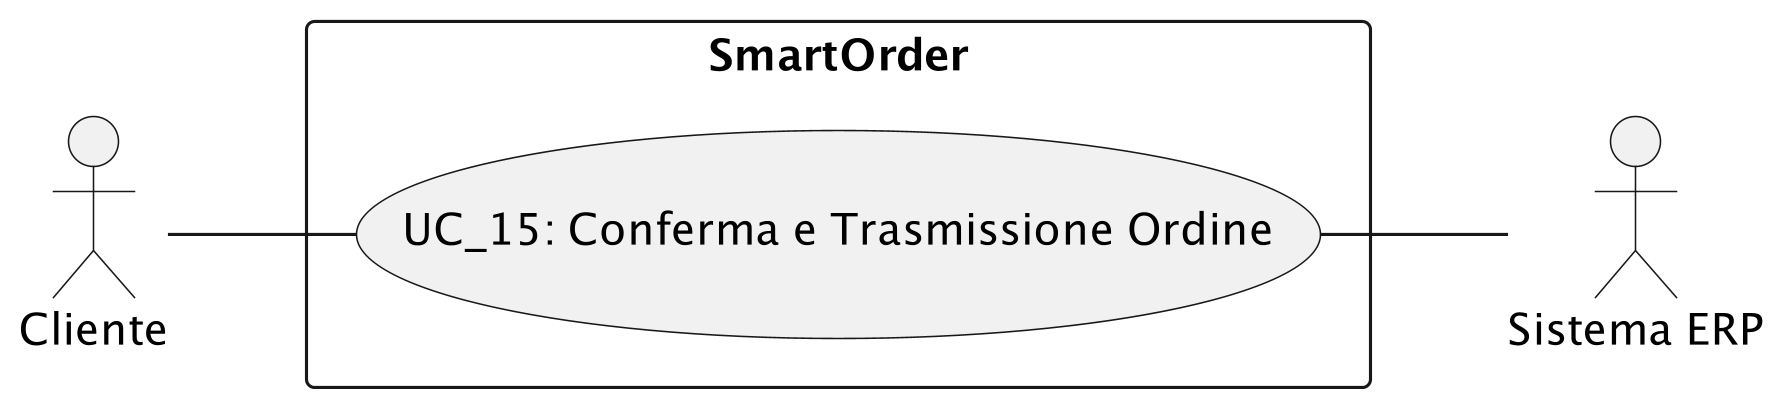
\includegraphics[width=0.8\textwidth]{uc-15.png}
    \caption{UC\_15: Conferma e Trasmissione Ordine}
\end{figure}

\begin{itemize}
    \item \textbf{Attori}: Cliente (Attore Primario), Sistema ERP (Attore Secondario)
    \item \textbf{User Story}: Come Cliente, ritenendomi soddisfatto della lista creata, voglio richiedere la sottomissione formale della richiesta affinché venga processata a livello commerciale e logistico.
    \item \textbf{Scenario Principale}: 
    \begin{enumerate}
        \item Il Cliente richiede formalmente la finalizzazione attivando il controllo primario di checkout.
        \item Il backend incrocia e valida i codici con le logiche di business aziendali (compatibilità assortimentale, disponibilità inventario).
        \item Il sistema confeziona l'architettura dati dell'ordine formattandola in un file strutturato JSON.
        \item Il sistema trasmette o deposita attivamente il file presso il Sistema ERP aziendale, demandando a quest'ultimo la competenza su fatturazione e pricing.
    \end{enumerate}
    \item \textbf{Precondizioni}: La lista articoli conta almeno una referenza valida a database. Non vi sono ticket di assistenza pendenti o blocchi attivi per l'utenza corrente.
    \item \textbf{Postcondizioni}: I dati di carrello escono dal perimetro della webapp. La sessione viene ripulita e il Cliente viene instradato tramite routing automatico alla dashboard dello Storico Ordini.
    \item \textbf{Estensioni}:
    \begin{itemize}
        \item \textit{Blocco per violazione logica di business}: Durante la validazione (Punto 2), il sistema rileva un'anomalia critica (es. prodotto appena uscito dall'assortimento). Il processo di trasmissione viene abortito. Il routing viene annullato e le righe incriminate vengono marcate a schermo con un flag grafico, costringendo l'Utente a intervenire.
    \end{itemize}
    \item \textbf{Trigger}: Azione intenzionale del Cliente sul pulsante di completamento ordine.
\end{itemize}

% -------------------------------------------------------------------

\subsection{UC\_16: Visualizzazione Storico Ordini}
\label{uc_16}

\begin{figure}[H]
    \centering 
    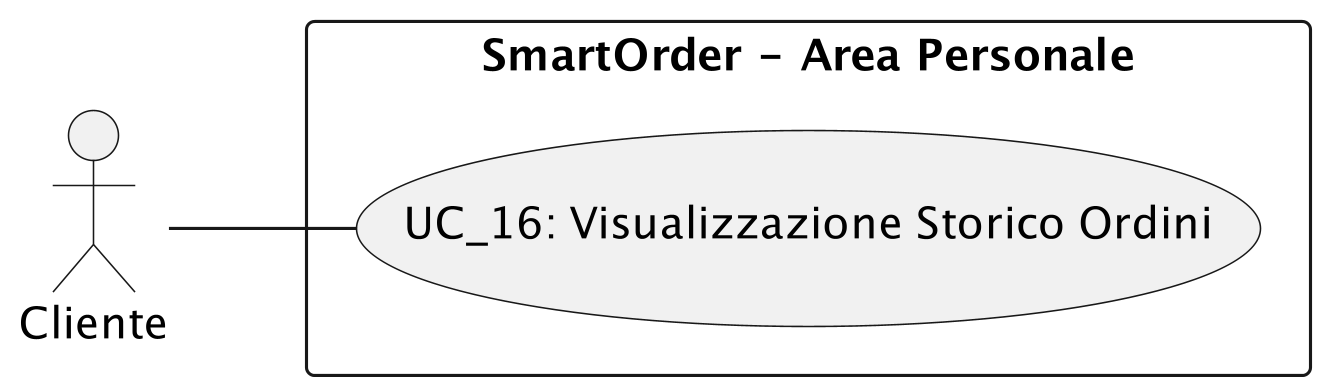
\includegraphics[width=0.7\textwidth]{uc-16.png}
    \caption{UC\_16: Visualizzazione Storico Ordini}
\end{figure}

\begin{itemize}
    \item \textbf{Attore Principale}: Cliente
    \item \textbf{User Story}: Come Cliente, voglio accedere a una lista cronologica di tutti gli ordini che ho effettuato in passato, affinché io possa consultare i miei volumi d'acquisto e ritrovare specifiche transazioni.
    \item \textbf{Scenario Principale}: 
    \begin{enumerate}
        \item Il Cliente richiede l'accesso all'area dedicata allo storico tramite l'apposito comando di navigazione.
        \item Il sistema interroga il database e recupera la lista degli ordini associati univocamente all'utenza corrente, ordinandoli in senso cronologico discendente (dal più recente).
        \item Il sistema itera sulla lista ed espone a schermo le singole transazioni, renderizzando per ciascuna:
        \begin{itemize}
            \item L'ID e la data dell'ordine.
            \item Il numero totale di prodotti ordinati.
            \item Un'anteprima dei primi 3 prodotti dell'ordine (nome del prodotto e quantità).
        \end{itemize}
    \end{enumerate}
    \item \textbf{Precondizioni}: Il Cliente possiede una sessione attiva. Esiste almeno un record storico associato al suo identificativo.
    \item \textbf{Postcondizioni}: La lista degli ordini pregressi è visibile in sola lettura. Se il Cliente vi accede immediatamente dopo un checkout (\hyperref[uc_15]{UC\_15}), l'ordine appena generato appare transitoriamente evidenziato in cima alla lista.
    \item \textbf{Trigger}: Selezione del comando di navigazione verso lo storico ordini.
\end{itemize}

% -------------------------------------------------------------------

\subsection{UC\_17: Esportazione Storico Ordini (Formato CSV\textsubscript{\textsc{g}})}
\label{uc_17}

\begin{figure}[H]
    \centering 
    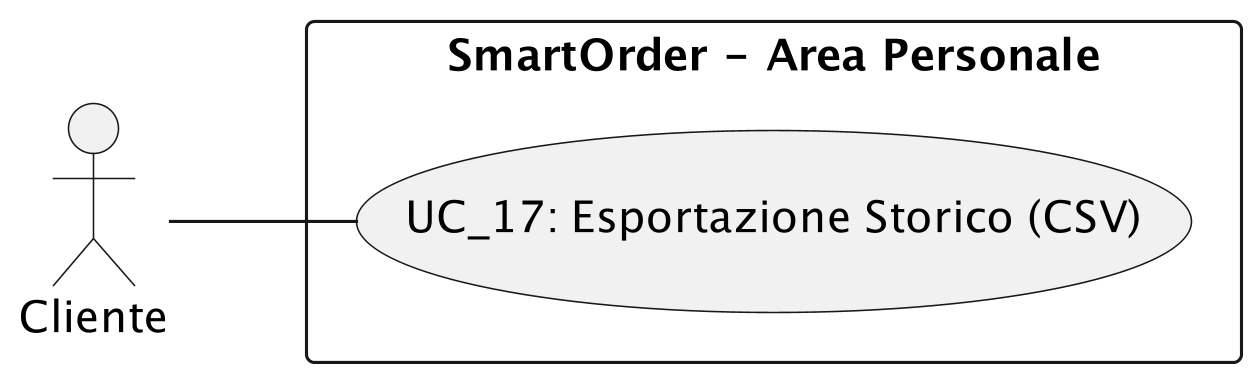
\includegraphics[width=0.7\textwidth]{uc-17.png}
    \caption{UC\_17: Esportazione Storico Ordini (Formato CSV)}
\end{figure}

\begin{itemize}
    \item \textbf{Attore Principale}: Cliente
    \item \textbf{Nota Requisito}: Questa funzionalità è classificata come requisito desiderabile.
    \item \textbf{User Story}: Come Cliente, voglio poter scaricare l'intero database dei miei ordini in un formato tabellare standard, per poterli archiviare, importare ed elaborare nel mio gestionale interno o su fogli di calcolo.
    \item \textbf{Scenario Principale}: 
    \begin{enumerate}
        \item Il Cliente innesca la richiesta di esportazione dati tramite l'apposito comando (es. bottone "Scarica storico acquisti").
        \item Il sistema interroga il database ed estrae lo storico completo degli ordini associati al Cliente.
        \item Il sistema formatta i dati estratti generando dinamicamente un file strutturato in formato CSV (Comma-Separated Values).
        \item Il sistema forza l'apertura di un flusso di download verso il dispositivo locale del Cliente.
    \end{enumerate}
    \item \textbf{Precondizioni}: Il Cliente possiede una sessione attiva. Il database contiene almeno un ordine storicizzato per quell'utenza.
    \item \textbf{Postcondizioni}: Il sistema operativo del client intercetta il flusso e salva il file \textit{.csv} nel File System locale. Lo stato dei dati sul database della webapp rimane inalterato.
    \item \textbf{Trigger}: Azione intenzionale del Cliente sul controllo globale di esportazione dati.
\end{itemize}
% -------------------------------------------------------------------

\subsection{UC\_18: Ispezione Dettaglio Ordine (Lato Cliente)}
\label{uc_18}

\begin{figure}[H]
    \centering 
    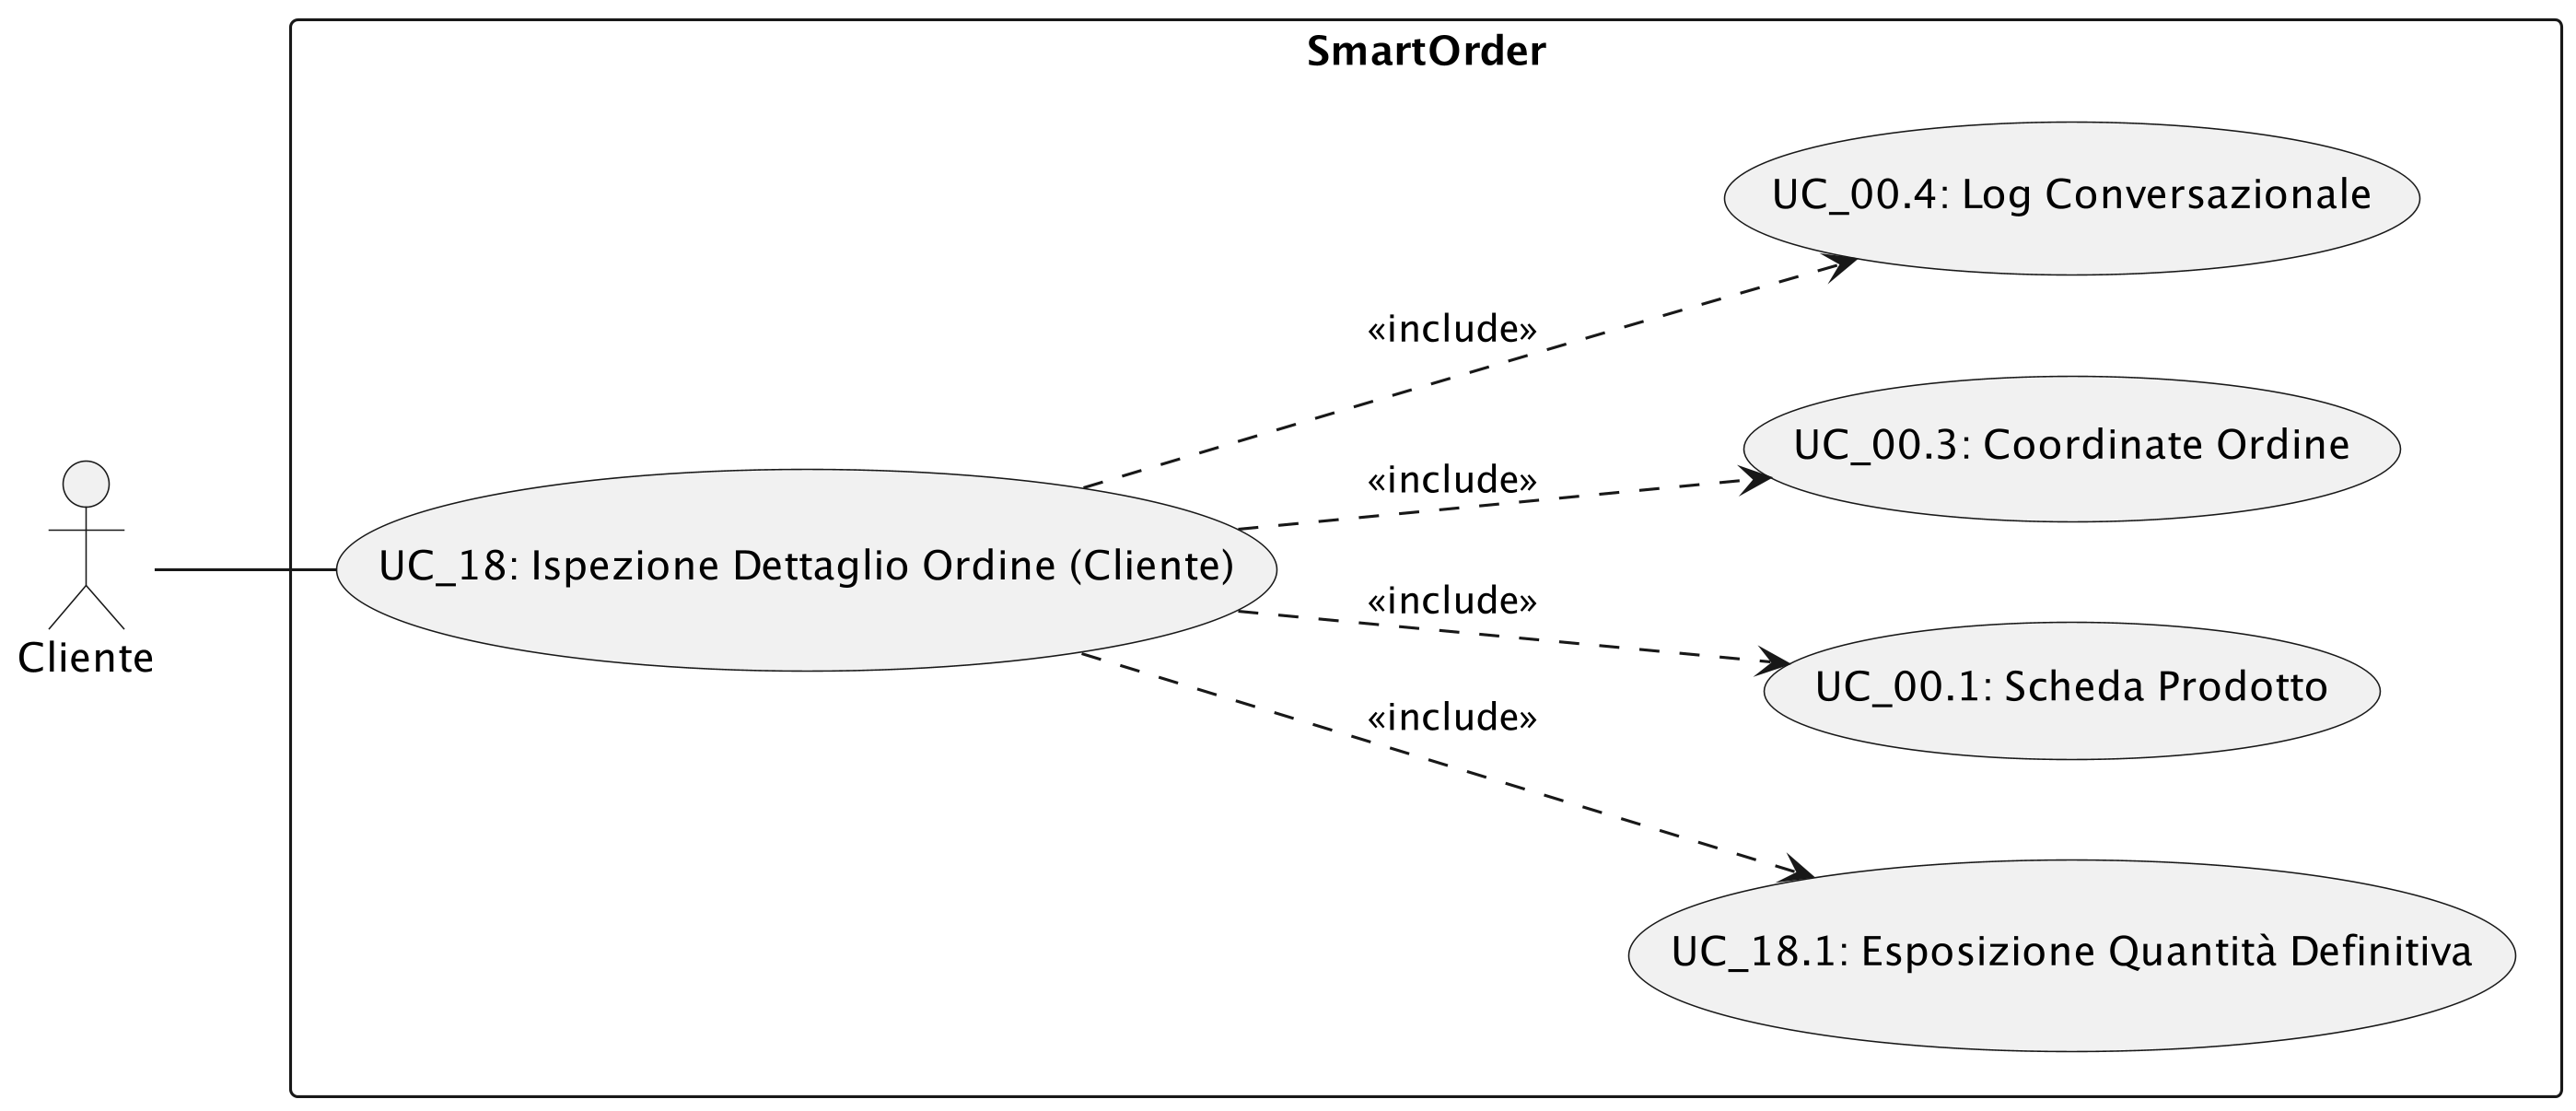
\includegraphics[width=0.8\textwidth]{uc-18.png}
    \caption{UC\_18: Visualizzazione Dettaglio Ordine}
\end{figure}

\begin{itemize}
    \item \textbf{Attore Principale}: Cliente
    \item \textbf{User Story}: Come Cliente, selezionando un ordine pregresso, voglio accedere a una vista approfondita che mi mostri l'elenco completo dei prodotti acquistati e la cronologia della conversazione che ha generato quel carrello.
    \item \textbf{Scenario Principale}: 
    \begin{enumerate}
        \item Il Cliente attiva il comando di espansione su uno specifico blocco riepilogativo dello Storico (\hyperref[uc_16]{UC\_16}).
        \item Il sistema istanzia la vista di dettaglio dedicata alla transazione.
        \item Il sistema espone le coordinate cardinali per inquadrare il documento $\rightarrow$ Include: \hyperref[uc_00.3]{UC\_00.3}
        \item Il sistema inietta il log storico della conversazione $\rightarrow$ Include: \hyperref[uc_00.4]{UC\_00.4}
        \item Per ogni articolo consolidato in quel checkout, il sistema ne espone la scheda anagrafica $\rightarrow$ Include: \hyperref[uc_00.1]{UC\_00.1}
        \item Per ogni articolo, viene affiancata la quantità storicizzata $\rightarrow$ Vedi \hyperref[uc_18.1]{UC\_18.1}
    \end{enumerate}
    \item \textbf{Precondizioni}:
    \begin{itemize}
        \item Il Cliente naviga nello Storico e attiva un record logicamente valido e associato al suo identificativo.
    \end{itemize}
    \item \textbf{Postcondizioni}:
    \begin{itemize}
        \item L'intero perimetro informativo dell'ordine (prodotti e chat) viene esposto in modalità di sola lettura (Read-Only). Nessuna operazione di modifica commerciale è ammessa, in quanto i dati risiedono già sotto l'autorità dell'ERP esterno.
    \end{itemize}
    \item \textbf{Inclusioni}:
    \begin{itemize}
        \item \hyperref[uc_00.1]{UC\_00.1}, \hyperref[uc_00.3]{UC\_00.3}, \hyperref[uc_00.4]{UC\_00.4}, \hyperref[uc_18.1]{UC\_18.1}
    \end{itemize}
    \item \textbf{Trigger}: Interazione fisica sul record di un ordine in elenco.
\end{itemize}

\subsubsection{UC\_18.1: Esposizione Quantità Definitiva}
\label{uc_18.1}
\begin{itemize}
    \item \textbf{Attore Principale}: Cliente
    \item \textbf{Scenario Principale}: A integrazione dei metadati logistici forniti da \hyperref[uc_00.1]{UC\_00.1}, il sistema espone il numero esatto di unità inviate al gestionale per quello specifico prodotto al momento del checkout.
    \item \textbf{Postcondizioni}: Il valore numerico viene renderizzato in formato testo, privo di qualsiasi controllo di iterazione incrementale o decrementale (impossibilità di alterazione).
\end{itemize}

% -------------------------------------------------------------------
% ==========================================
% GRUPPO F: ASSISTENZA E HUMAN HANDOFF
% ==========================================

\subsection{UC\_19: Apertura Ticket Assistenza}
\label{uc_19}

\begin{figure}[H]
    \centering 
    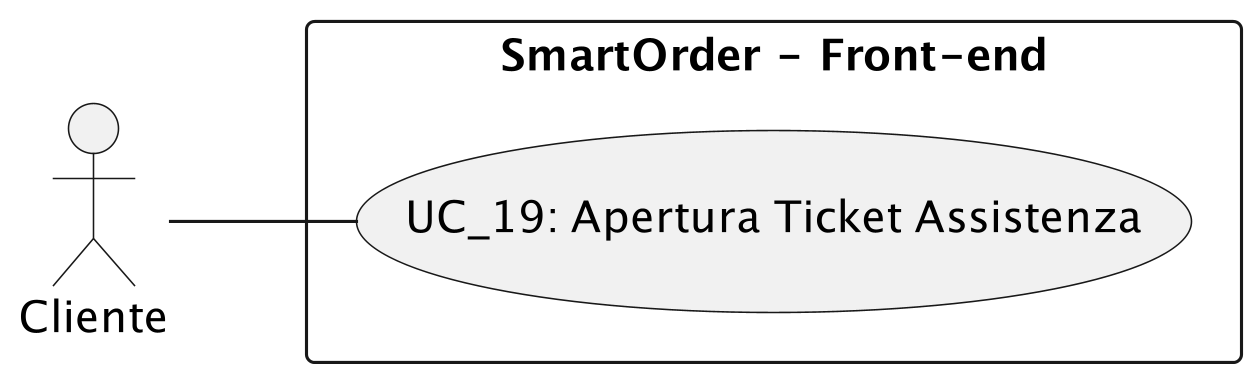
\includegraphics[width=0.6\textwidth]{uc-19.png}
    \caption{Apertura Ticket Assistenza}
\end{figure}

\begin{itemize}
    \item \textbf{Attore Principale}: Cliente
    \item \textbf{User Story}: Come Cliente, se riscontro difficoltà nell'interazione con l'AI, voglio poter richiedere l'intervento di un operatore umano che subentri nella sessione per aiutarmi a completare l'ordine.
    \item \textbf{Scenario Principale}: 
    \begin{enumerate}
        \item Il Cliente attiva la funzione di assistenza tramite l'apposito controllo nell'interfaccia principale.
        \item Il sistema sospende istantaneamente l'elaborazione autonoma dell'AI per la sessione corrente.
        \item Il sistema genera un avviso automatico in chat informando il Cliente dell'imminente arrivo di un operatore e invitandolo a descrivere il problema.
        \item L'interfaccia muta dinamicamente: viene inibita la funzione di "Nuova Sessione" e il comando di richiesta assistenza viene sostituito dal comando di "Chiusura Assistenza".
        \item Il sistema genera e accoda una notifica (Ticket in stato "Aperto") nella dashboard globale del backoffice.
    \end{enumerate}
    \item \textbf{Precondizioni}: Il Cliente ha una sessione di composizione ordine attiva. Non sono presenti altre richieste di assistenza pendenti per la medesima sessione.
    \item \textbf{Postcondizioni}: Lo stato della sessione è marcato come "In Assistenza". L'AI è silenziata. Il controllo degli input conversazionali (\hyperref[uc_07]{UC\_07}, \hyperref[uc_08]{UC\_08}) passa all'interazione tra Cliente e Operatore.
    \item \textbf{Trigger}: Selezione del comando di richiesta intervento umano.
\end{itemize}

% -------------------------------------------------------------------

\subsection{UC\_20: Chiusura Ticket di Assistenza}
\label{uc_20}

\begin{figure}[H]
    \centering 
    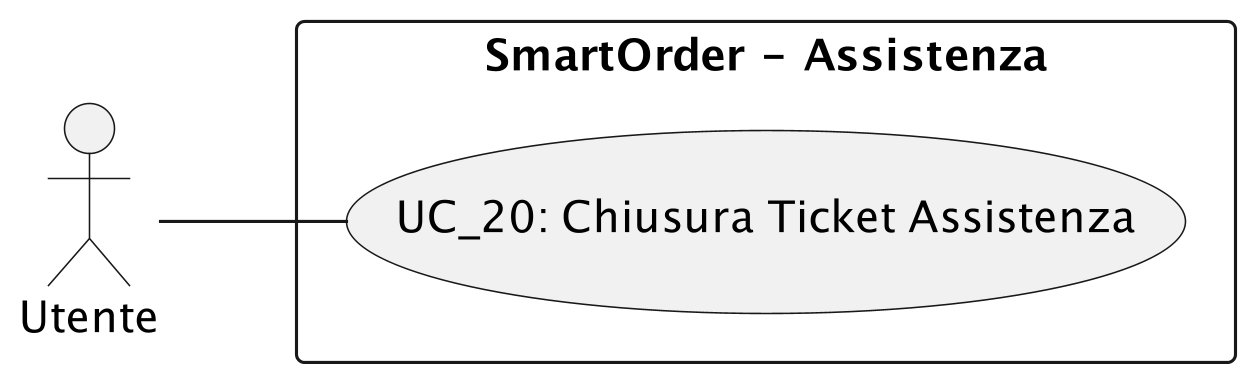
\includegraphics[width=0.7\textwidth]{uc-20.png}
    \caption{UC\_20: Chiusura Ticket di Assistenza}
\end{figure}

\begin{itemize}
    \item \textbf{Attore Principale}: Utente
    \item \textbf{User Story}: Come Utente loggato (Cliente nel front-end o Operatore nel backoffice), voglio poter chiudere formalmente il ticket di assistenza una volta che la problematica è stata risolta, per ripristinare il normale funzionamento autonomo della piattaforma.
    \item \textbf{Scenario Principale}:
    \begin{enumerate}
        \item L'Utente invoca il comando di chiusura del ticket di assistenza tramite l'apposito controllo d'interfaccia.
        \item Il sistema aggiorna lo stato del record associato al Ticket in "Chiuso" a livello di database.
        \item Il sistema riattiva il motore di elaborazione semantica dell'LLM, restituendogli il dominio esclusivo sui successivi input conversazionali.
        \item Il sistema aggiorna dinamicamente le interfacce coinvolte:
        \begin{itemize}
            \item \textbf{Lato Cliente}: Vengono ripristinati i controlli operativi standard (abilitazione del comando "Nuova Sessione") e viene iniettato un log testuale in chat per certificare la conclusione dell'intervento umano.
            \item \textbf{Lato Operatore}: La finestra di interazione diretta viene dismessa e il ticket scompare dalla coda delle lavorazioni attive.
        \end{itemize}
    \end{enumerate}
    \item \textbf{Precondizioni}: Esiste un ticket associato alla sessione corrente formalmente in stato "Aperto" o "In lavorazione".
    \item \textbf{Postcondizioni}: 
    \begin{itemize}
        \item \textbf{Stato Entità}: Il ciclo di vita del Ticket si conclude, consolidandosi definitivamente nello stato "Chiuso".
        \item \textbf{Gestione Permessi}: Viene revocato il token di subentro; l'Operatore perde ogni privilegio di visualizzazione e modifica sul carrello e sulla chat del Cliente.
        \item \textbf{Ripristino Automazione}: Il dominio operativo della sessione viene restituito in via esclusiva all'Intelligenza Artificiale, ripristinando il normale ciclo di gestione automatica.
    \end{itemize}
    \item \textbf{Trigger}: Selezione del comando di chiusura ticket.
\end{itemize}
% -------------------------------------------------------------------

\subsection{UC\_21: Consultazione Tabella Ticket Aperti}
\label{uc_21}

\begin{figure}[H]
    \centering 
    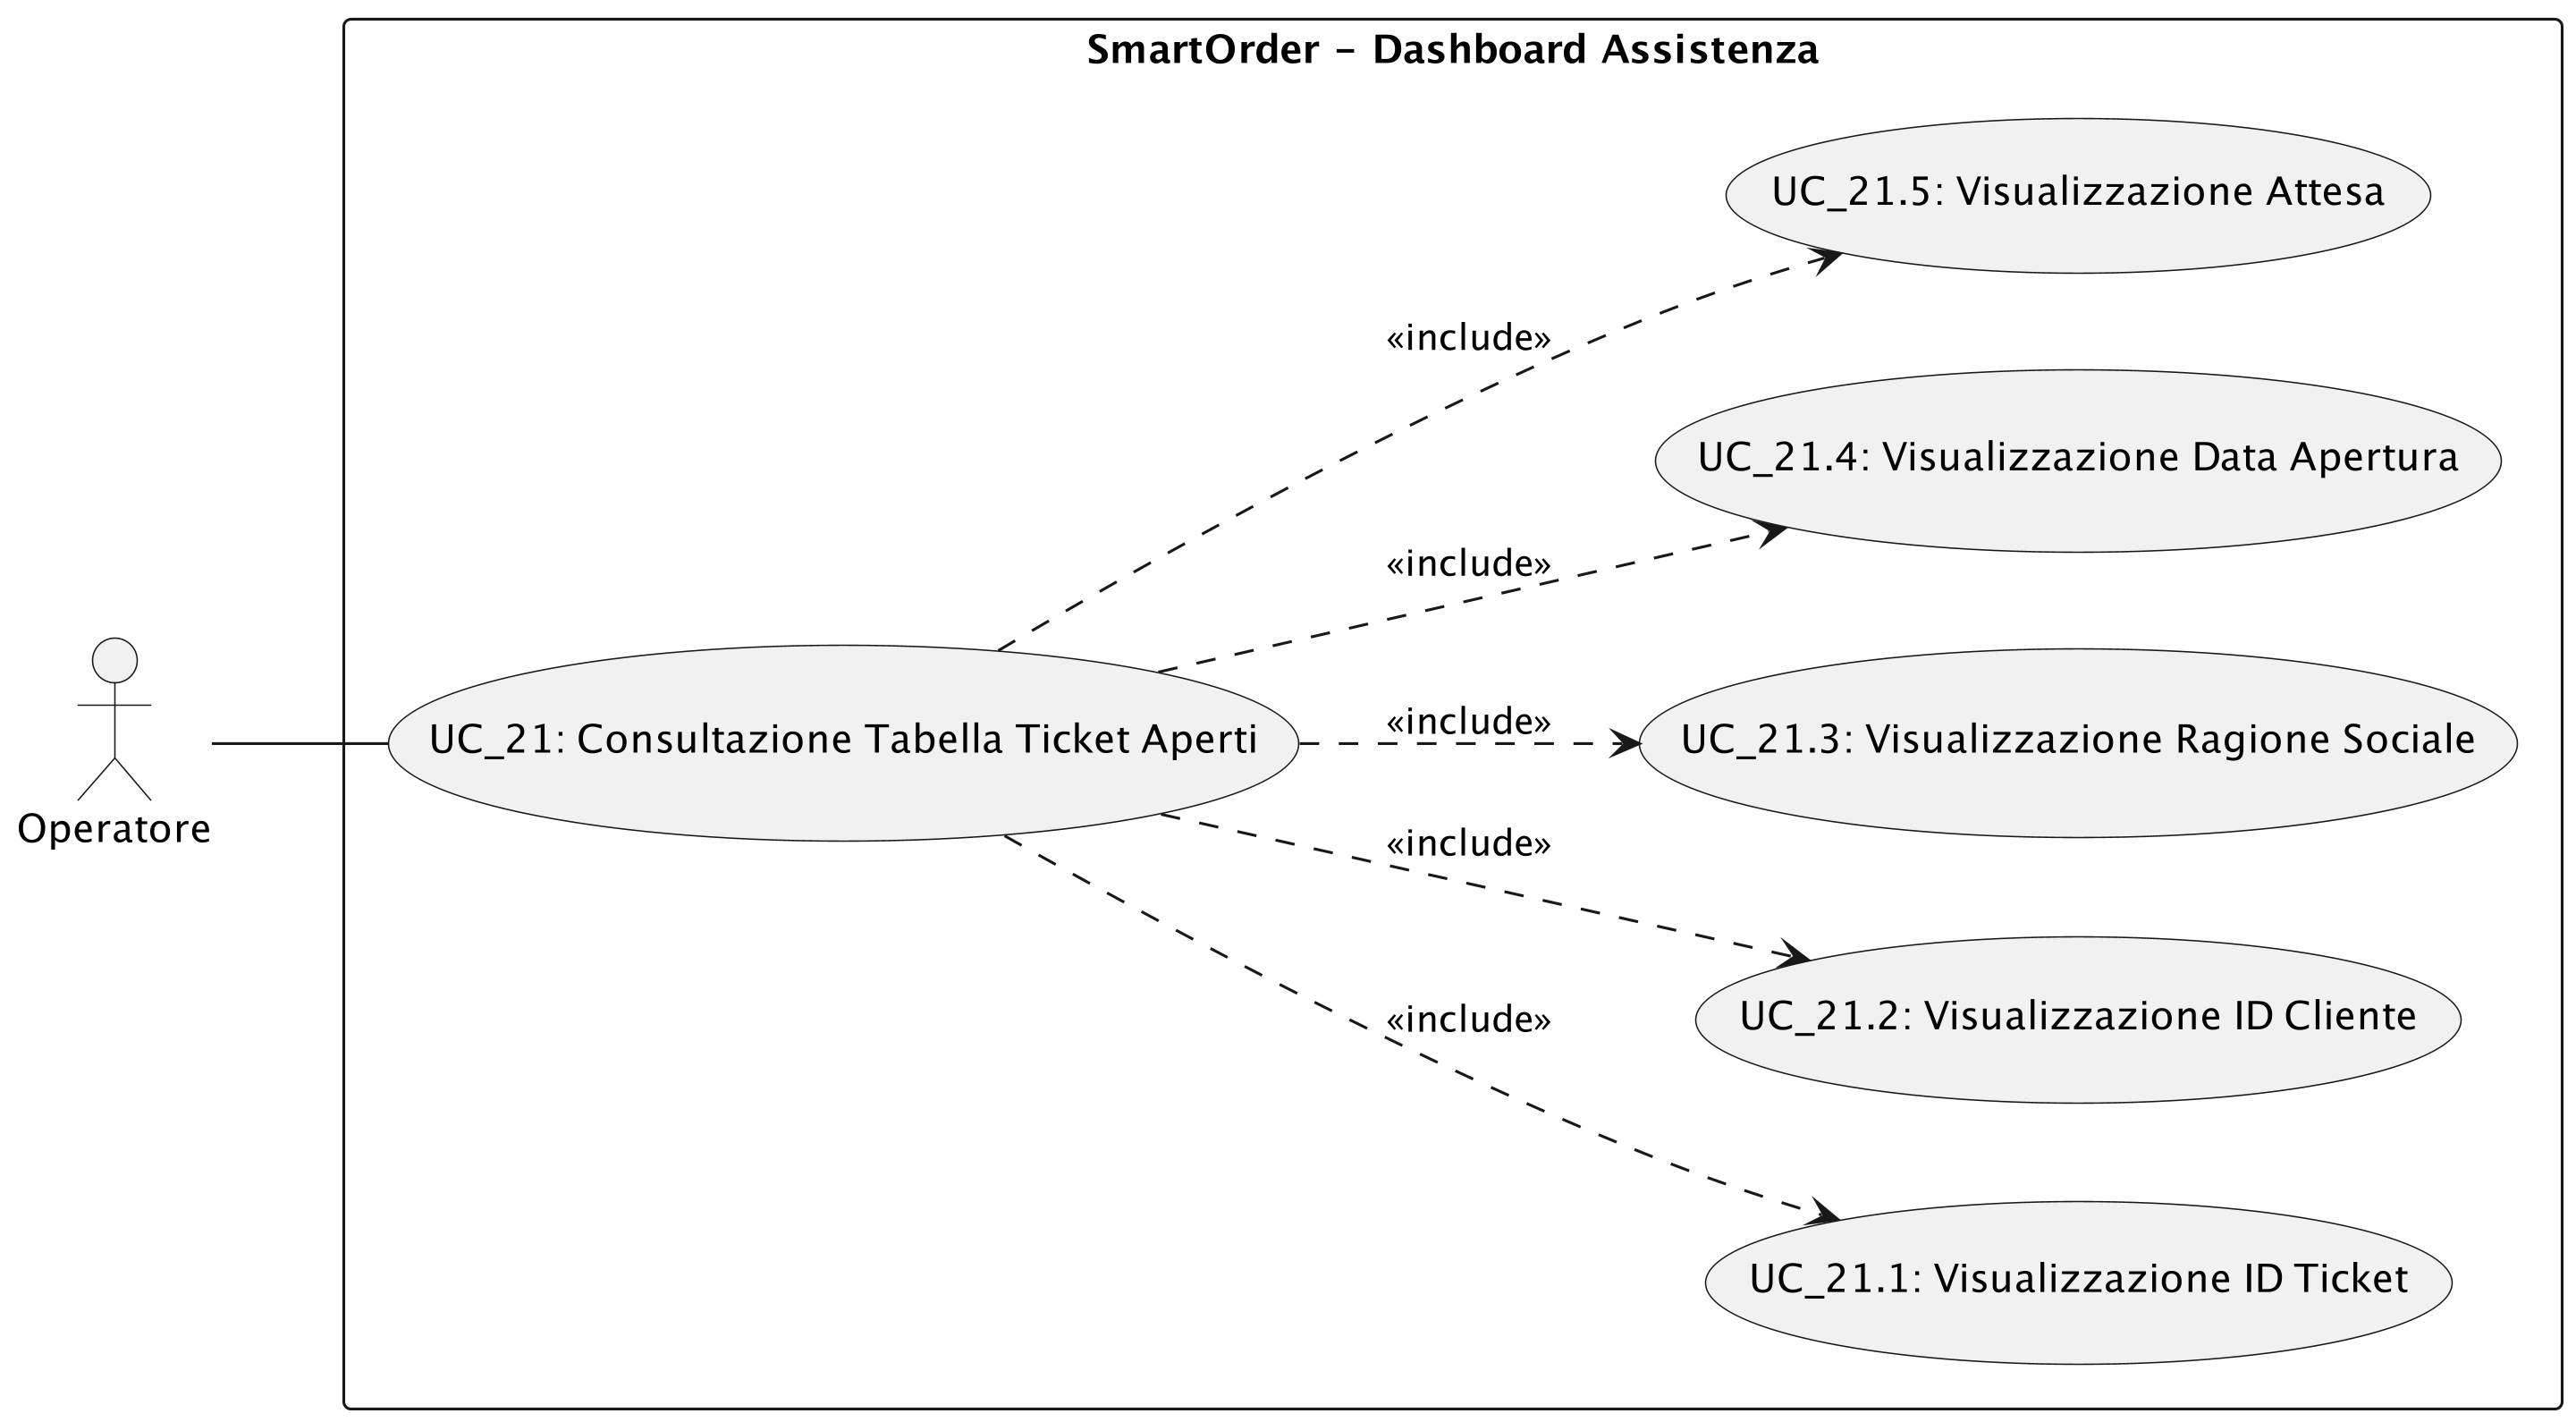
\includegraphics[width=0.7\textwidth]{uc-21.png} 
    \caption{UC\_21: Consultazione Tabella Ticket Aperti}
\end{figure}

\begin{itemize}
    \item \textbf{Attore Principale}: Operatore
    \item \textbf{User Story}: Come Operatore, voglio visualizzare la lista dei ticket di assistenza in sospeso, affinché io possa individuare rapidamente le richieste più urgenti o quelle di uno specifico cliente.
    \item \textbf{Scenario Principale}: 
    \begin{enumerate}
        \item L'Operatore accede alla dashboard dedicata all'assistenza.
        \item Il sistema interroga il database e recupera i record dei ticket in stato "Aperto" o "In lavorazione".
        \item Il sistema renderizza la tabella ordinando di default i record per tempo di attesa discendente.
        \item Per ogni ticket, esposizione ID Ticket $\rightarrow$ Include: \hyperref[uc_21.1]{UC\_21.1}
        \item Per ogni ticket, esposizione ID Cliente $\rightarrow$ Include: \hyperref[uc_21.2]{UC\_21.2}
        \item Per ogni ticket, esposizione Ragione Sociale $\rightarrow$ Include: \hyperref[uc_21.3]{UC\_21.3}
        \item Per ogni ticket, esposizione Data Apertura $\rightarrow$ Include: \hyperref[uc_21.4]{UC\_21.4}
        \item Per ogni ticket, esposizione Attesa differenziale $\rightarrow$ Include: \hyperref[uc_21.5]{UC\_21.5}
    \end{enumerate}
    \item \textbf{Precondizioni}: L'Operatore ha effettuato l'accesso al backoffice con i privilegi necessari.
    \item \textbf{Postcondizioni}: L'interfaccia mostra l'elenco aggiornato dei ticket in attesa di lavorazione.
    \item \textbf{Inclusioni}: \hyperref[uc_21.1]{UC\_21.1}, \hyperref[uc_21.2]{UC\_21.2}, \hyperref[uc_21.3]{UC\_21.3}, \hyperref[uc_21.4]{UC\_21.4}, \hyperref[uc_21.5]{UC\_21.5}
    \item \textbf{Estensioni (Manipolazione della Vista e Azioni Asincrone)}:
    \begin{itemize}
        \item \textit{Ordinamento Dinamico}: L'Operatore clicca sull'intestazione della colonna "Tempo di attesa" per invertire l'ordine dei risultati (ascendente/discendente).
        \item \textit{Filtraggio Temporale}: L'Operatore seleziona un intervallo di date dal calendario; il sistema aggiorna la tabella omettendo i ticket fuori da quel periodo.
        \item \textit{Ricerca Mirata}: L'Operatore seleziona una colonna specifica e digita un testo; il sistema filtra istantaneamente la vista mostrando solo i record corrispondenti.
        \item \textit{Ricezione aggiornamenti (Live Sync)}: Se il backend registra un nuovo ticket, il sistema lo inietta istantaneamente nella tabella preservando l'ordinamento e i filtri attivi.
        \item \textit{Passaggio alla Gestione}: L'Operatore clicca su un record per aprire la console modale e avviare l'assistenza $\rightarrow$ Vedi \hyperref[uc_22]{UC\_22}.
    \end{itemize}
    \item \textbf{Trigger}: Navigazione dell'Operatore verso la dashboard "Ticket Aperti".
\end{itemize}

\subsubsection{UC\_21.1: Visualizzazione ID Ticket}
\label{uc_21.1}
\begin{itemize}
    \item \textbf{Attore Principale}: Operatore
    \item \textbf{Scenario Principale}: Il sistema preleva ed espone nella colonna preposta il codice alfanumerico univoco di sistema associato alla specifica richiesta di supporto.
\end{itemize}

\subsubsection{UC\_21.2: Visualizzazione ID Cliente}
\label{uc_21.2}
\begin{itemize}
    \item \textbf{Attore Principale}: Operatore
    \item \textbf{Scenario Principale}: Il sistema espone il codice anagrafico gestionale afferente al Cliente che ha innescato l'escalation.
\end{itemize}

\subsubsection{UC\_21.3: Visualizzazione Ragione Sociale}
\label{uc_21.3}
\begin{itemize}
    \item \textbf{Attore Principale}: Operatore
    \item \textbf{Scenario Principale}: Il sistema risolve la chiave esterna e preleva dalla tabella anagrafica locale la denominazione estesa dell'azienda, rendendola visibile in tabella.
\end{itemize}

\subsubsection{UC\_21.4: Visualizzazione Data Apertura Ticket}
\label{uc_21.4}
\begin{itemize}
    \item \textbf{Attore Principale}: Operatore
    \item \textbf{Scenario Principale}: Il sistema recupera e formatta in un formato cronologico leggibile (es. gg/mm/aaaa hh:mm) il timestamp esatto di genesi della richiesta.
\end{itemize}

\subsubsection{UC\_21.5: Visualizzazione Attesa dall'ultimo messaggio}
\label{uc_21.5}
\begin{itemize}
    \item \textbf{Attore Principale}: Operatore
    \item \textbf{Scenario Principale}: Il sistema calcola matematicamente il differenziale temporale rispetto all'istante di ricezione dell'ultimo input inviato dal Cliente e lo formatta a video sotto forma di sintesi testuale (es. "5 min").
\end{itemize}

% ==========================================
% GRUPPO G: GESTIONE TICKET (OPERATORE)
% ==========================================

\subsection{UC\_22: Gestione Ticket (Subentro Modale)}
\label{uc_22}

\begin{figure}[H]
    \centering 
    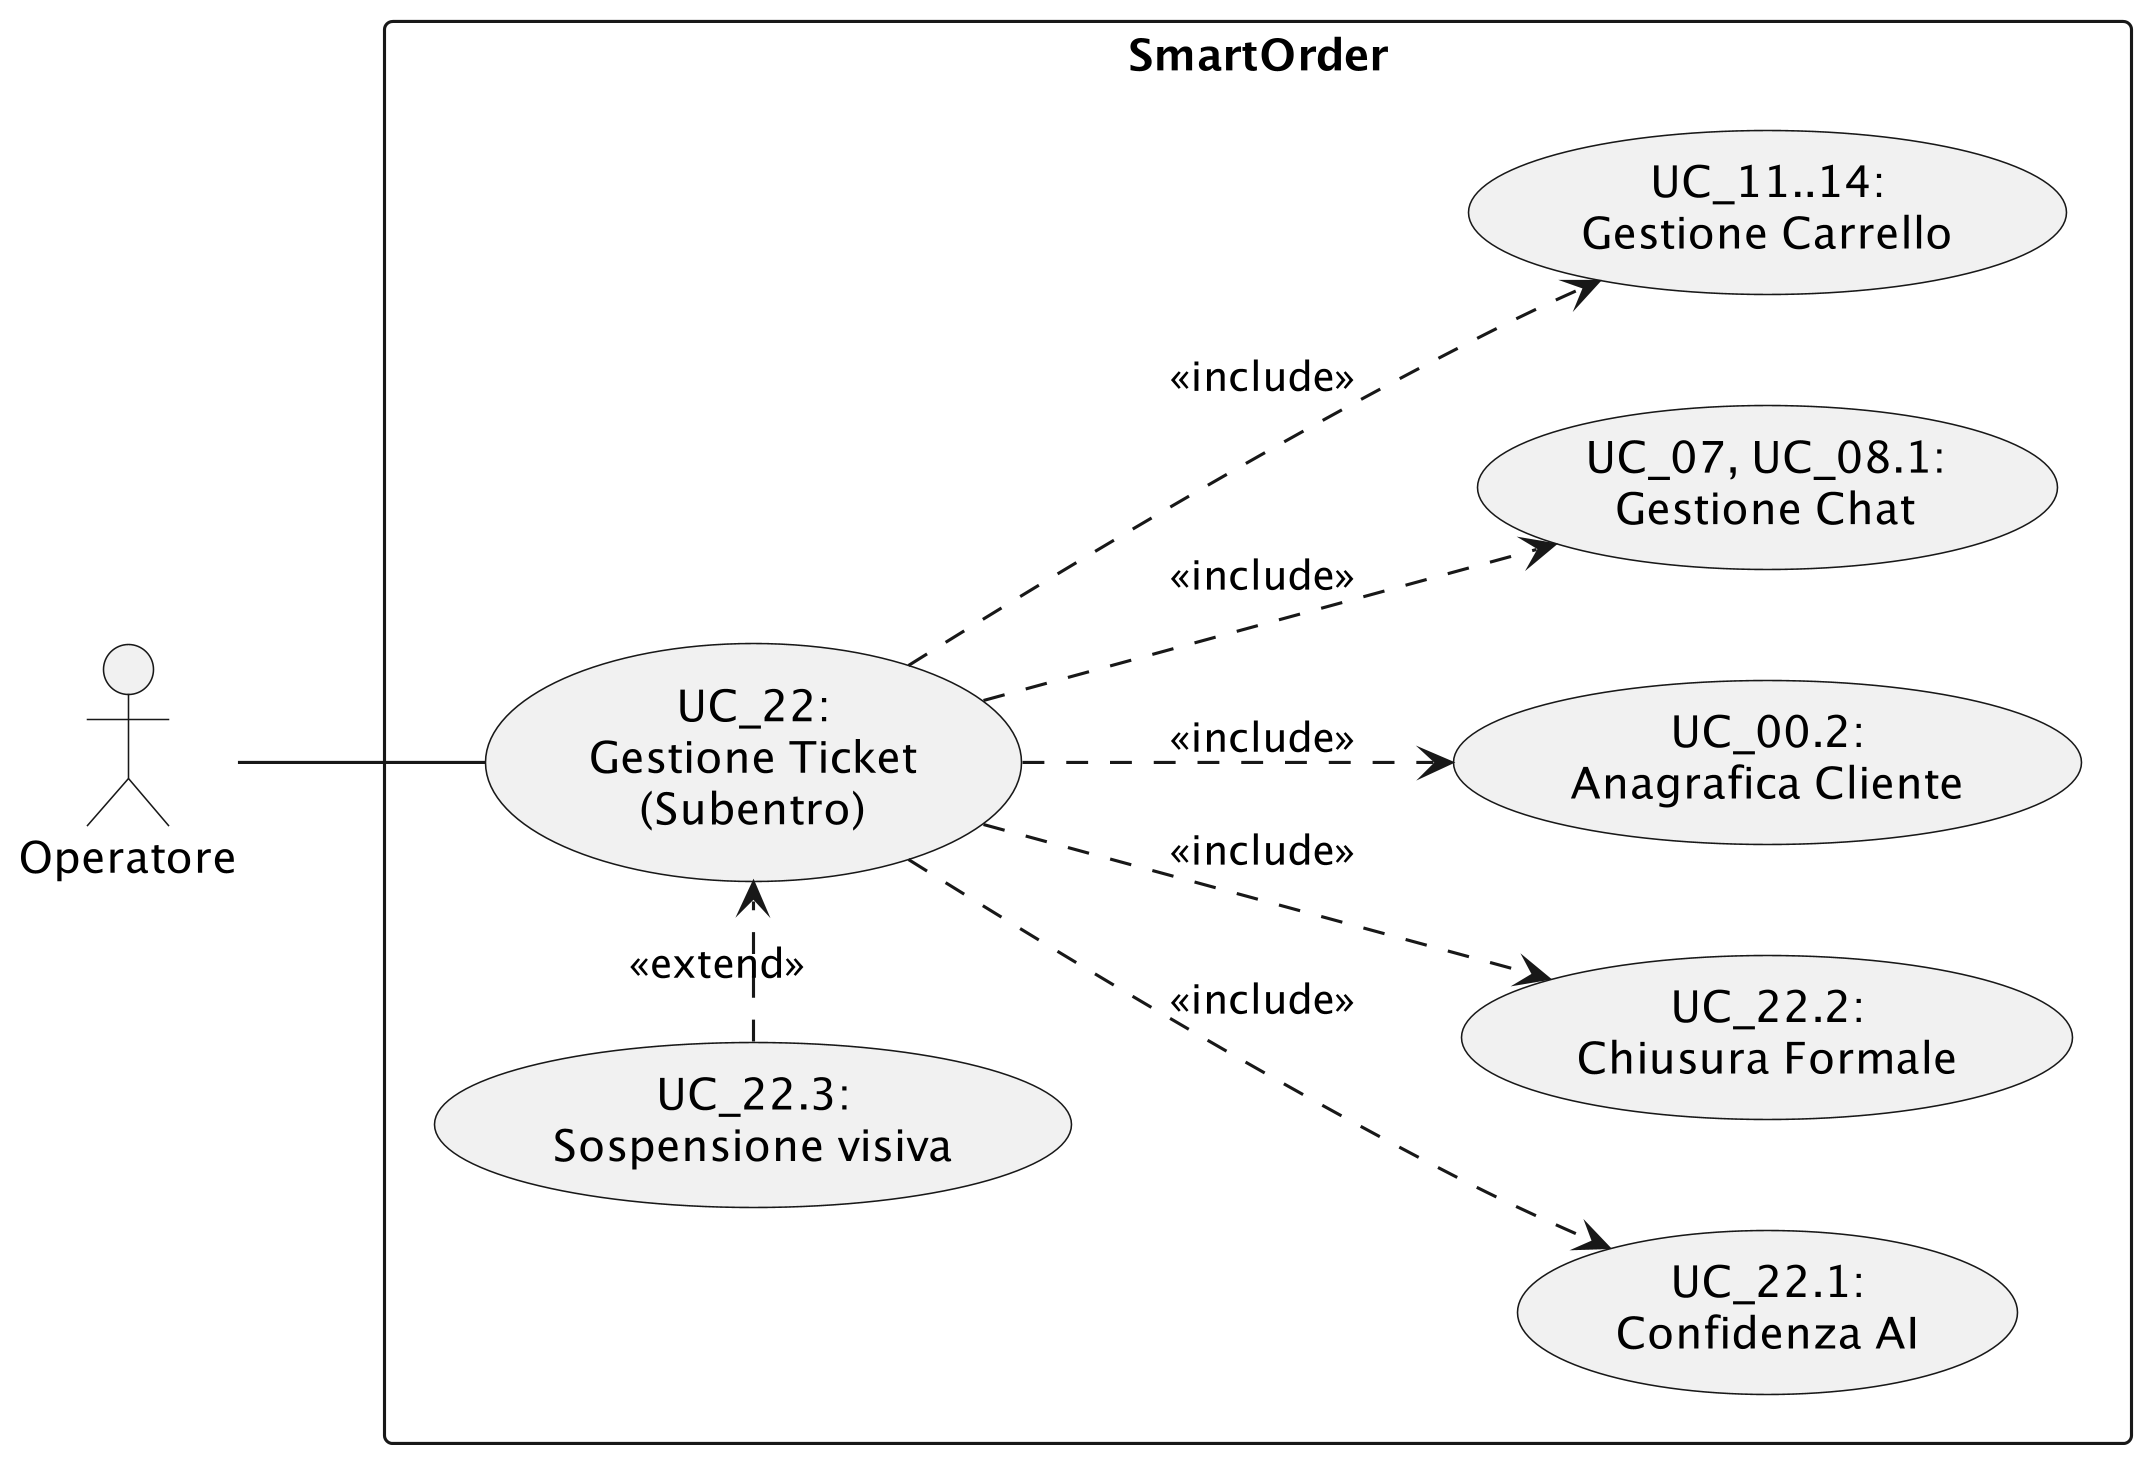
\includegraphics[width=0.8\textwidth]{uc-22.png}
    \caption{UC\_22: Gestione Ticket (Subentro Modale)}
\end{figure}

\begin{itemize}
    \item \textbf{Attore Principale}: Operatore
    \item \textbf{User Story}: Come Operatore, voglio avere a disposizione una console protetta in cui posso subentrare nella sessione di un Cliente per dirimere anomalie, comunicando con esso e manipolando i volumi del suo carrello da remoto.
    \item \textbf{Scenario Principale}: 
    \begin{enumerate}
        \item Il sistema intercetta l'apertura del ticket, registra l'assegnazione logica esclusiva (Lock) sull'Operatore ed espone la console in sovraimpressione (Modal).
        \item Il sistema inietta nell'intestazione le coordinate anagrafiche del Cliente $\rightarrow$ Include: \hyperref[uc_00.2]{UC\_00.2}
        \item Il sistema espone il flusso di comunicazione in tempo reale $\rightarrow$ Include: \hyperref[uc_07]{UC\_07}
        \item L'Operatore interagisce immettendo testo a supporto del Cliente $\rightarrow$ Include: \hyperref[uc_08.1]{UC\_08.1}
        \item L'Operatore manipola il carrello in delega (ricerca cataloghi, aggiunta logica, modifica quantità, rimozione) avvalendosi dei componenti standard di piattaforma $\rightarrow$ Include: \hyperref[uc_11]{UC\_11}, \hyperref[uc_12]{UC\_12}, \hyperref[uc_13]{UC\_13}, \hyperref[uc_14]{UC\_14}
        \item Contestualmente al carrello, esposizione del Livello di Confidenza AI $\rightarrow$ Vedi \hyperref[uc_22.1]{UC\_22.1}
        \item Chiusura formale della pratica $\rightarrow$ Vedi \hyperref[uc_22.2]{UC\_22.2}
    \end{enumerate}
    \item \textbf{Precondizioni}:
    \begin{itemize}
        \item L'Operatore si trova nella tabella "Ticket Aperti" e interagisce con un record in stato "Aperto" attualmente privo di Lock concorrente (nessun altro collega vi sta operando).
    \end{itemize}
    \item \textbf{Postcondizioni}:
    \begin{itemize}
        \item L'Operatore assume e mantiene il pieno controllo asincrono (Read/Write) sui dati di sessione del Cliente. Le variazioni applicate vengono salvate contestualmente nel DB del carrello remoto. Al termine, il Lock di sistema viene rilasciato.
    \end{itemize}
    \item \textbf{Inclusioni}:
    \begin{itemize}
        \item \hyperref[uc_00.2]{UC\_00.2}, \hyperref[uc_07]{UC\_07}, \hyperref[uc_08.1]{UC\_08.1}
        \item \hyperref[uc_11]{UC\_11}, \hyperref[uc_12]{UC\_12}, \hyperref[uc_13]{UC\_13}, \hyperref[uc_14]{UC\_14}
        \item \hyperref[uc_22.1]{UC\_22.1}, \hyperref[uc_22.2]{UC\_22.2}
    \end{itemize}
    \item \textbf{Estensioni}:
    \begin{itemize}
        \item Sospensione visiva temporanea dell'interfaccia $\rightarrow$ Vedi \hyperref[uc_22.3]{UC\_22.3}
    \end{itemize}
    \item \textbf{Trigger}: Selezione deliberata di un record interagibile dalla tabella di backoffice.
\end{itemize}

\subsubsection{UC\_22.1: Visualizzazione Livello di Confidenza AI}
\label{uc_22.1}
\begin{itemize}
    \item \textbf{Attore Principale}: Operatore
    \item \textbf{Scenario Principale}: A integrazione della visualizzazione standard del carrello (\hyperref[uc_13]{UC\_13}), il sistema espone contestualmente per ogni riga processata dall'Intelligenza Artificiale il relativo parametro di affidabilità (Confidence Score percentuale).
    \item \textbf{Postcondizioni}: L'Operatore dispone di una metrica tecnica e diagnostica, la cui visualizzazione resta rigorosamente invisibile ed esclusa dall'interfaccia pubblica del Cliente.
\end{itemize}

\subsubsection{UC\_22.2: Chiusura Formale Ticket}
\label{uc_22.2}
\begin{itemize}
    \item \textbf{Attore Principale}: Operatore
    \item \textbf{Scenario Principale}: L'Operatore innesca il comando di dismissione definitiva. Il database archivia lo stato in "Chiuso" ed esegue la revoca totale del token di Lock.
    \item \textbf{Postcondizioni}: Il sistema riabilita automaticamente le funzionalità di checkout sul terminale remoto del Cliente (comunicando il termine del subentro) e smonta l'istanza della console per l'Operatore.
\end{itemize}

\subsubsection{UC\_22.3: Sospensione visiva dell'interfaccia (Estensione)}
\label{uc_22.3}
\begin{itemize}
    \item \textbf{Attore Principale}: Operatore
    \item \textbf{Scenario Principale}: L'Operatore attiva il comando di chiusura contestuale (es. logica off-canvas o collasso visivo del layer modale). Il componente UI viene nascosto senza attuare procedure distruttive sui dati immessi.
    \item \textbf{Postcondizioni}: Il sistema mantiene rigorosamente inalterato lo stato "Aperto" del ticket e preserva il Lock di sicurezza sull'Operatore, permettendo a quest'ultimo l'ispezione protetta della dashboard sottostante o l'accesso ad altri moduli del gestionale per reperire informazioni.
\end{itemize}

% ==========================================
% GRUPPO H: GESTIONE STORICO ORDINI (OPERATORE)
% ==========================================

\subsection{UC\_23: Consultazione Storico Ordini Globale}
\label{uc_23}

\begin{figure}[H]
    \centering 
    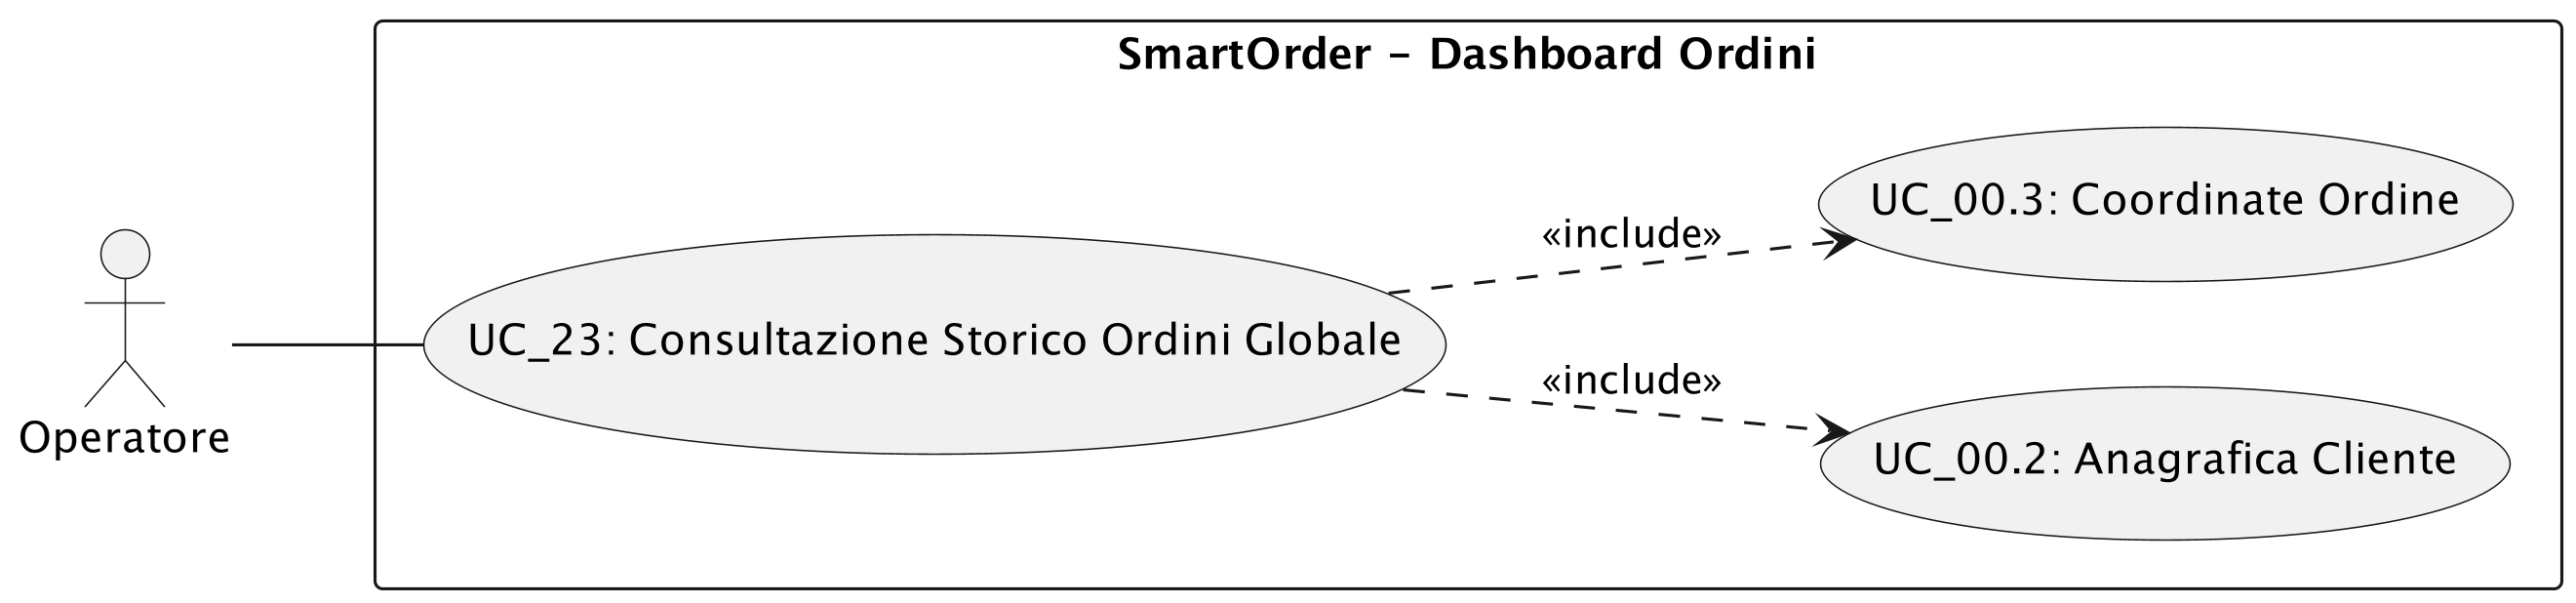
\includegraphics[width=0.7\textwidth]{uc-23.png}
    \caption{UC\_23: Consultazione Storico Ordini Globale}
\end{figure}

\begin{itemize}
    \item \textbf{Attore Principale}: Operatore
    \item \textbf{User Story}: Come Operatore, voglio poter visualizzare una vista riepilogativa contenente lo storico globale degli ordini effettuati da tutti i clienti, affinché io possa monitorare il flusso transazionale in piattaforma.
    \item \textbf{Scenario Principale}: 
    \begin{enumerate}
        \item L'Operatore accede alla dashboard dedicata allo storico ordini globale.
        \item Il sistema interroga il database e recupera l'elenco dei record transazionali.
        \item Il sistema renderizza la tabella ordinando di default i record per data di transazione discendente.
        \item Per ogni ordine esposto, esposizione delle coordinate temporali e di sistema $\rightarrow$ Include: \hyperref[uc_00.3]{UC\_00.3}.
        \item Per ogni ordine esposto, esposizione dell'anagrafica aziendale associata $\rightarrow$ Include: \hyperref[uc_00.2]{UC\_00.2}.
    \end{enumerate}
    \item \textbf{Precondizioni}: L'Operatore ha effettuato l'accesso al backoffice con i privilegi necessari.
    \item \textbf{Postcondizioni}: L'interfaccia mostra l'elenco aggiornato degli ordini a sistema.
    \item \textbf{Inclusioni}: \hyperref[uc_00.2]{UC\_00.2}, \hyperref[uc_00.3]{UC\_00.3}
    \item \textbf{Estensioni (Manipolazione della Vista e Azioni Asincrone)}:
    \begin{itemize}
        \item \textit{Ordinamento Dinamico}: L'Operatore clicca sull'intestazione di una colonna per invertire l'ordine dei risultati (ascendente/discendente).
        \item \textit{Filtraggio Temporale}: L'Operatore seleziona un intervallo di date dal calendario; il sistema aggiorna la tabella omettendo gli ordini fuori da quel periodo.
        \item \textit{Ricerca Mirata}: L'Operatore seleziona una colonna specifica (es. "Cliente") e digita un testo; il sistema filtra istantaneamente la vista mostrando solo i record corrispondenti.
        \item \textit{Ricezione aggiornamenti (Live Sync)}: Se il backend registra il checkout di un nuovo ordine, il sistema inietta istantaneamente il record in cima alla tabella.
        \item \textit{Ispezione Dettaglio}: L'Operatore clicca su un record della tabella per aprire la scheda di dettaglio in sovraimpressione $\rightarrow$ Vedi \hyperref[uc_24]{UC\_24}.
    \end{itemize}
    \item \textbf{Trigger}: Navigazione dell'Operatore verso la dashboard "Ordini".
\end{itemize}

% -------------------------------------------------------------------

\subsection{UC\_24: Ispezione Dettaglio Ordine Globale}
\label{uc_24}

\begin{figure}[H]
    \centering 
    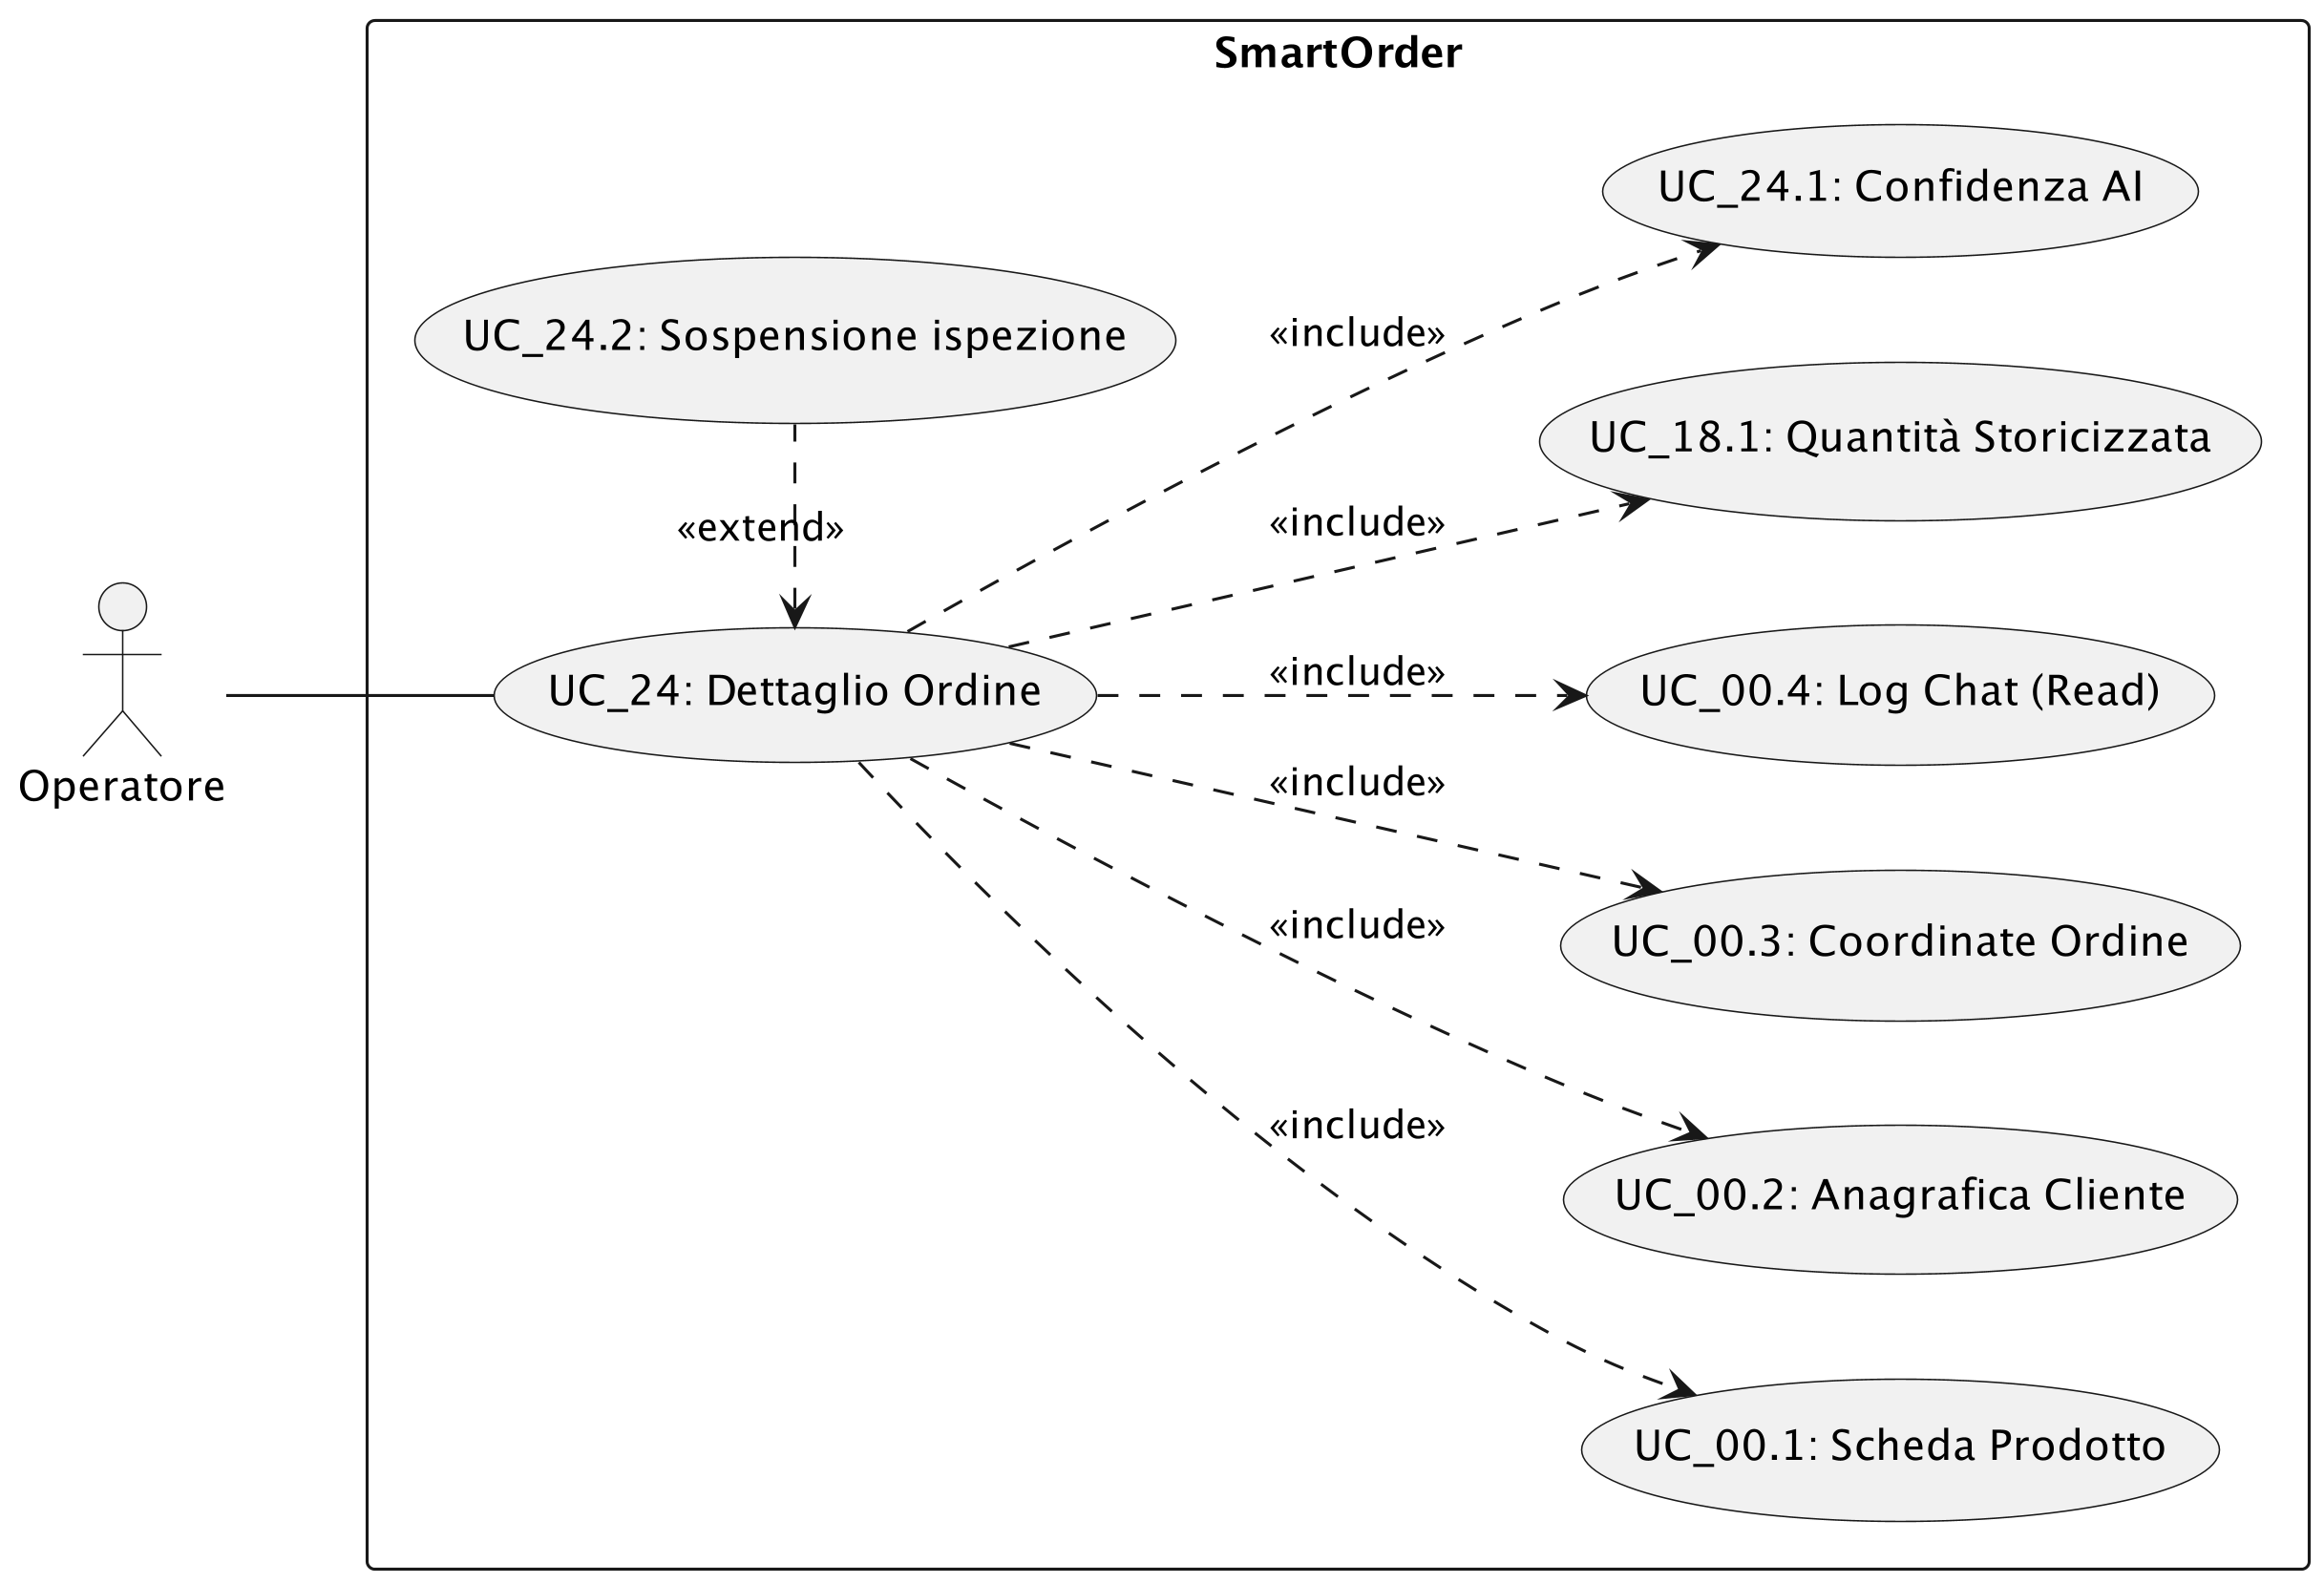
\includegraphics[width=0.8\textwidth]{uc-24.png}
    \caption{UC\_24: Ispezione Dettaglio Ordine Globale}
\end{figure}

\begin{itemize}
    \item \textbf{Attore Principale}: Operatore
    \item \textbf{User Story}: Come Operatore, voglio aprire una scheda approfondita dell'ordine per ispezionarne il contenuto logistico e il contesto conversazionale originario.
    \item \textbf{Scenario Principale}: 
    \begin{enumerate}
        \item Il sistema istanzia l'interfaccia dedicata ai dettagli dell'ordine in sovraimpressione (Modal).
        \item Esposizione coordinate generali e anagrafica Cliente $\rightarrow$ Include: \hyperref[uc_00.2]{UC\_00.2}, \hyperref[uc_00.3]{UC\_00.3}
        \item Esposizione log conversazionale storico $\rightarrow$ Include: \hyperref[uc_00.4]{UC\_00.4}
        \item Per ogni riga d'ordine, esposizione dei metadati prodotto $\rightarrow$ Include: \hyperref[uc_00.1]{UC\_00.1}
        \item Per ogni riga d'ordine, esposizione della quantità definitiva $\rightarrow$ Include: \hyperref[uc_18.1]{UC\_18.1}
        \item Esposizione Livello Confidenza AI $\rightarrow$ Vedi \hyperref[uc_24.1]{UC\_24.1}
    \end{enumerate}
    \item \textbf{Precondizioni}:
    \begin{itemize}
        \item La tabella "Ordini" (\hyperref[uc_23]{UC\_23}) è attiva e l'Operatore ha interagito con un record valido.
    \end{itemize}
    \item \textbf{Postcondizioni}:
    \begin{itemize}
        \item Il sistema espone il dettaglio completo dell'ordine e il log conversazionale in modalità puramente consultiva, garantendo l'assoluta immutabilità dello storico. Si ribadisce l'assenza di dati legati al pricing, delegati all'ERP esterno.
    \end{itemize}
    \item \textbf{Inclusioni}:
    \begin{itemize}
        \item \hyperref[uc_00.1]{UC\_00.1}, \hyperref[uc_00.2]{UC\_00.2}, \hyperref[uc_00.3]{UC\_00.3}, \hyperref[uc_00.4]{UC\_00.4}, \hyperref[uc_18.1]{UC\_18.1}, \hyperref[uc_24.1]{UC\_24.1}
    \end{itemize}
    \item \textbf{Estensioni}:
    \begin{itemize}
        \item Sospensione dell'ispezione visiva $\rightarrow$ Vedi \hyperref[uc_24.2]{UC\_24.2}
    \end{itemize}
    \item \textbf{Trigger}: L'Operatore attiva il comando di ispezione espandendo un record specifico della tabella.
\end{itemize}

\subsubsection{UC\_24.1: Visualizzazione Livello di Confidenza AI}
\label{uc_24.1}
\begin{itemize}
    \item \textbf{Attore Principale}: Operatore
    \item \textbf{Scenario Principale}: A corredo della riga prodotto, il sistema preleva il metadato valutativo originato dall'LLM al momento dell'interpretazione semantica e lo esplicita graficamente per consentire all'Operatore verifiche diagnostiche sull'algoritmo.
\end{itemize}

\subsubsection{UC\_24.2: Sospensione dell'ispezione}
\label{uc_24.2}
\begin{itemize}
    \item \textbf{Attore Principale}: Operatore
    \item \textbf{Scenario Principale}: L'Operatore innesca il comando di chiusura contestuale.
    \item \textbf{Postcondizioni}: Il sistema smonta l'istanza grafica di dettaglio e ripristina il focus primario sulla vista tabellare principale.
\end{itemize}

% ==========================================
% GRUPPO I: OTTIMIZZAZIONE AI (HUMAN-IN-THE-LOOP)
% ==========================================

\subsection{UC\_25: Consultazione Log e Discrepanze AI}
\label{uc_25}

\begin{figure}[H]
    \centering 
    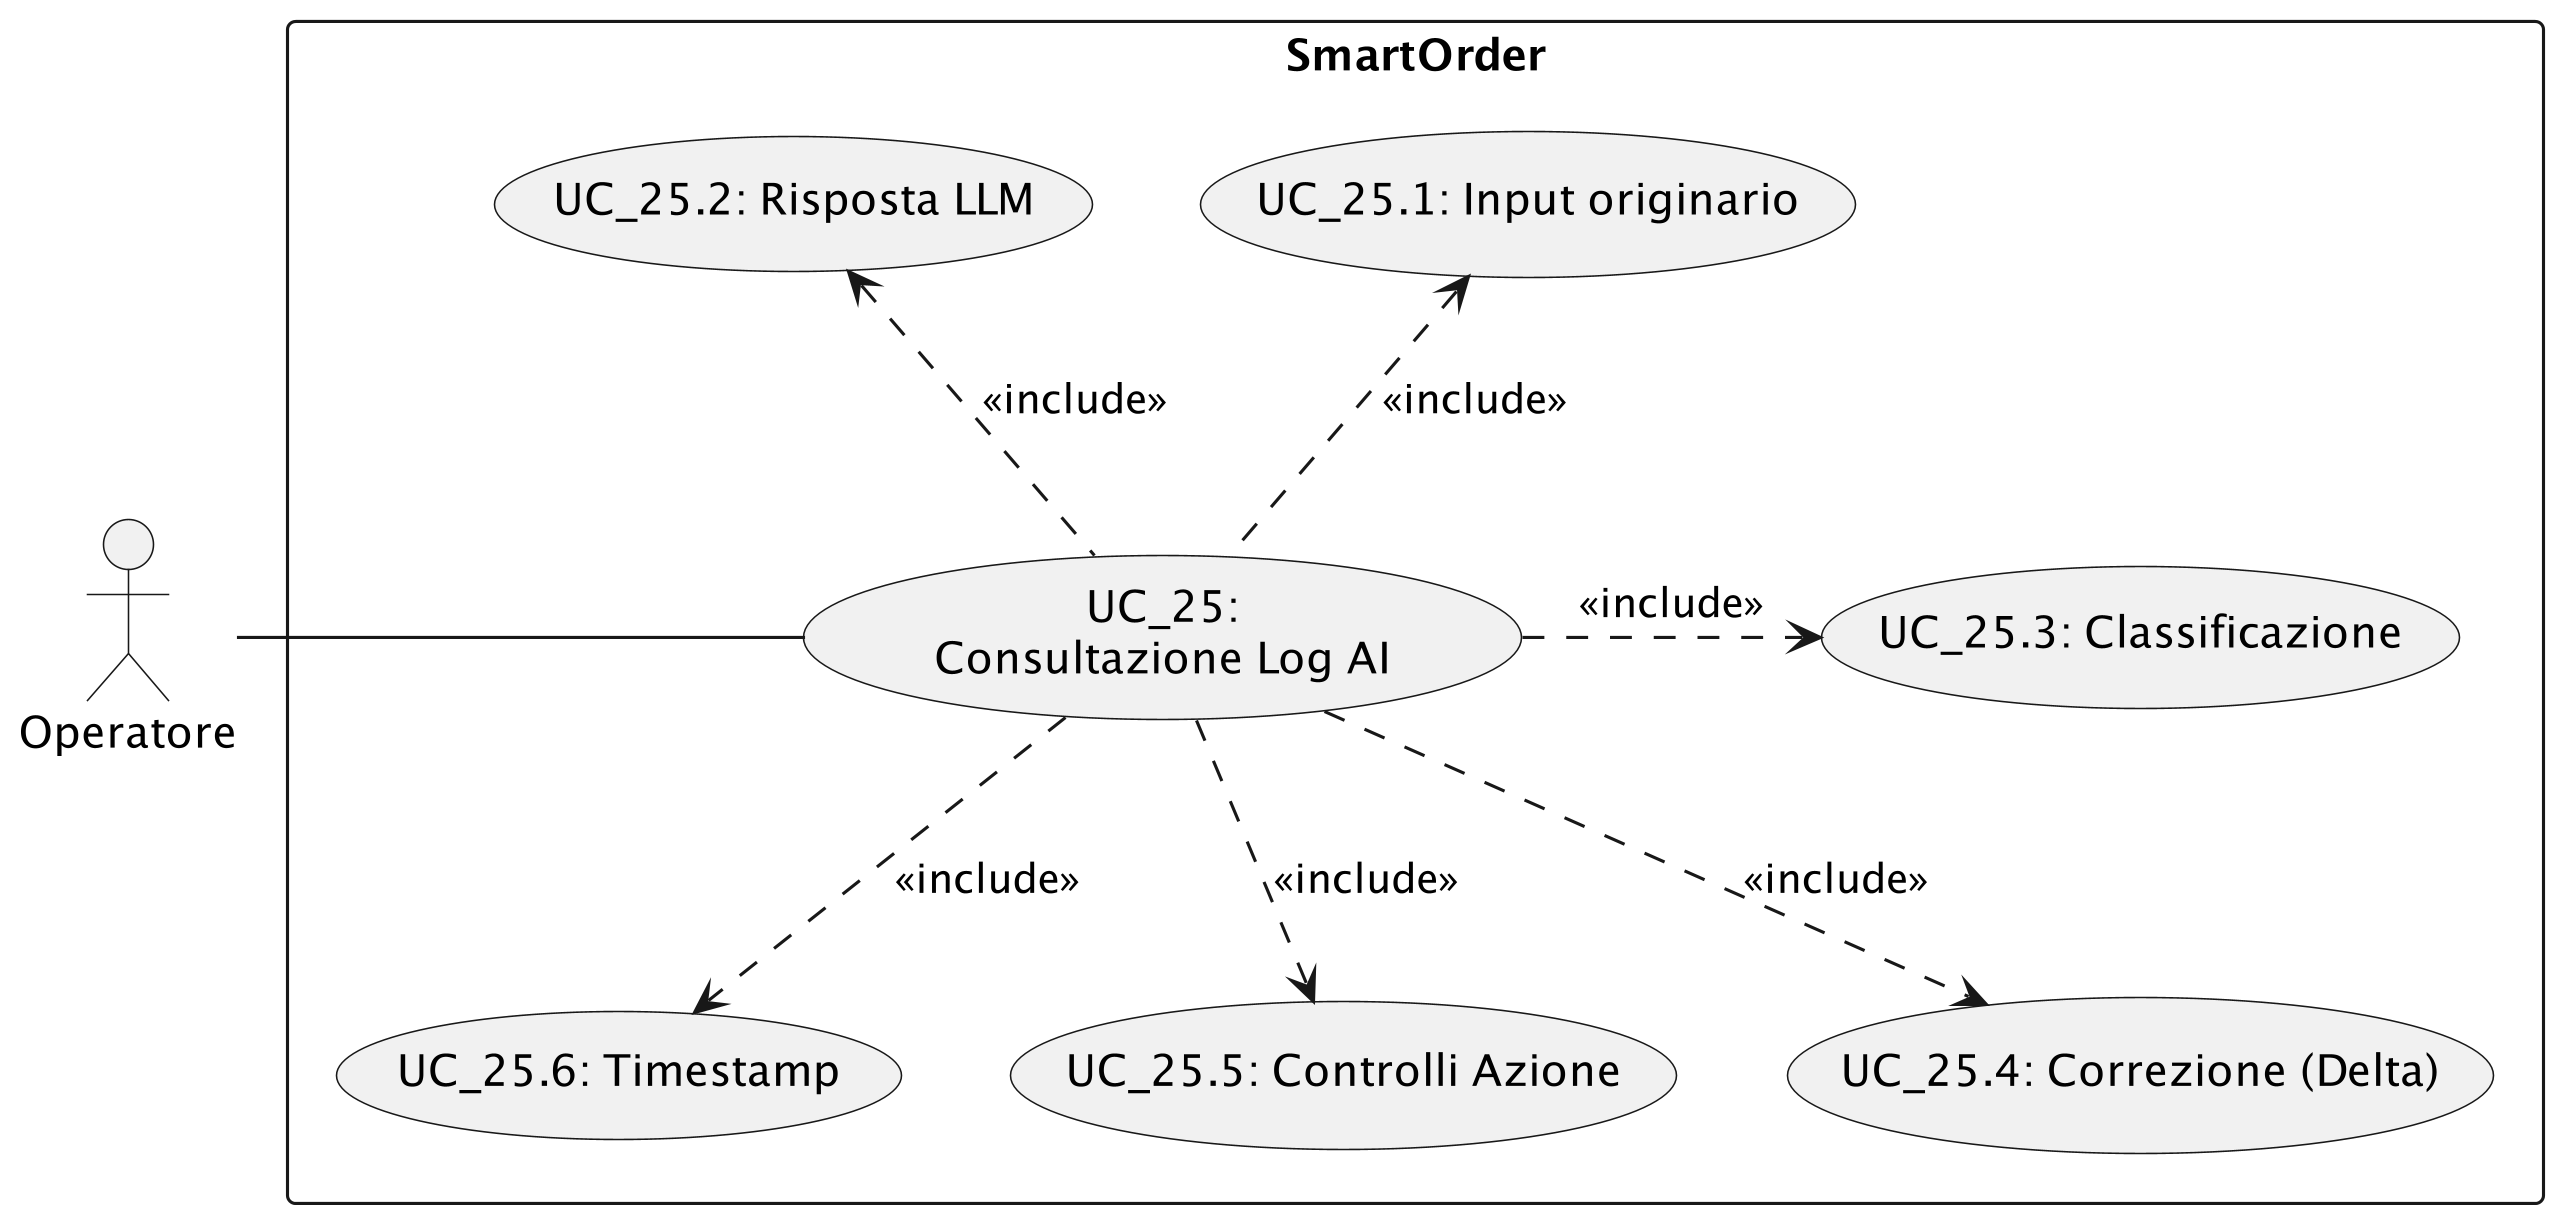
\includegraphics[width=0.7\textwidth]{uc-25.png}
    \caption{UC\_25: Consultazione Log e Discrepanze AI}
\end{figure}

\begin{itemize}
    \item \textbf{Attore Principale}: Operatore
    \item \textbf{User Story}: Come Operatore, voglio consultare una tabella contenente i record dei feedback negativi e delle correzioni manuali ai carrelli, affinché io possa analizzare gli errori dell'AI e valutare quali dati utilizzare per il successivo riaddestramento (Retraining\textsubscript{\textsc{g}}).
    \item \textbf{Scenario Principale}: 
    \begin{enumerate}
        \item L'Operatore accede alla dashboard dedicata all'Ottimizzazione AI.
        \item Il sistema interroga il database e recupera i log relativi alle discrepanze tra suggerimenti dell'AI e azioni effettive del Cliente.
        \item Il sistema renderizza la tabella ordinando i record per data e ora discendente (dal più recente al più vecchio).
        \item Per ogni record (Log), esposizione Input originario $\rightarrow$ Include: \hyperref[uc_25.1]{UC\_25.1}
        \item Per ogni record, esposizione Risposta LLM $\rightarrow$ Include: \hyperref[uc_25.2]{UC\_25.2}
        \item Per ogni record, esposizione Classificazione Utente $\rightarrow$ Include: \hyperref[uc_25.3]{UC\_25.3}
        \item Per ogni record, esposizione Correzione Rilevata (Delta) $\rightarrow$ Include: \hyperref[uc_25.4]{UC\_25.4}
        \item Per ogni record, esposizione Controlli di Azione $\rightarrow$ Include: \hyperref[uc_25.5]{UC\_25.5}
        \item Per ogni record, esposizione Timestamp $\rightarrow$ Include: \hyperref[uc_25.6]{UC\_25.6}
    \end{enumerate}
    \item \textbf{Precondizioni}: L'Operatore ha effettuato l'accesso al backoffice con i privilegi necessari per la gestione dei dati di addestramento.
    \item \textbf{Postcondizioni}: L'interfaccia espone l'elenco dei log. Di default, il sistema omette i record già processati (es. "Approvato" o "Scartato"), mostrando unicamente le segnalazioni in stato "Da gestire".
    \item \textbf{Inclusioni}: \hyperref[uc_25.1]{UC\_25.1}, \hyperref[uc_25.2]{UC\_25.2}, \hyperref[uc_25.3]{UC\_25.3}, \hyperref[uc_25.4]{UC\_25.4}, \hyperref[uc_25.5]{UC\_25.5}, \hyperref[uc_25.6]{UC\_25.6}
    \item \textbf{Estensioni (Manipolazione della Vista e Azioni Asincrone)}:
    \begin{itemize}
        \item \textit{Ordinamento Dinamico}: L'Operatore clicca sull'intestazione di una colonna per invertire l'ordine dei risultati esposti (ascendente/discendente).
        \item \textit{Filtraggio per Stato}: L'Operatore seleziona uno stato dal menu a tendina (es. "Mostra tutti", "Solo approvati"); il sistema aggiorna la vista includendo i record precedentemente omessi.
        \item \textit{Filtraggio Temporale}: L'Operatore seleziona un intervallo di date dal calendario; il sistema aggiorna la tabella omettendo i log generati fuori da quel periodo.
        \item \textit{Ricerca Globale Multi-Campo}: L'Operatore digita un testo nel campo di ricerca globale; il sistema esegue una ricerca full-text asincrona su tutti gli attributi testuali (es. input utente, risposta LLM) e filtra i record corrispondenti.
        \item \textit{Ricezione aggiornamenti (Live Sync)}: Se il sistema registra un nuovo log di discrepanza o feedback negativo, il record viene iniettato istantaneamente nella tabella, preservando l'ordinamento attivo.
    \end{itemize}
    \item \textbf{Trigger}: Navigazione dell'Operatore verso la dashboard "Ottimizzazione AI".
\end{itemize}

\subsubsection{UC\_25.1: Esposizione Input originario}
\label{uc_25.1}
\begin{itemize}
    \item \textbf{Attore Principale}: Operatore
    \item \textbf{Scenario Principale}: Il sistema estrae e rende consultabile la trascrizione testuale esatta derivata dalla sorgente utente (audio o testo) che ha scatenato l'inferenza.
\end{itemize}

\subsubsection{UC\_25.2: Esposizione Risposta LLM}
\label{uc_25.2}
\begin{itemize}
    \item \textbf{Attore Principale}: Operatore
    \item \textbf{Scenario Principale}: Il sistema renderizza il tracciato di output logico originato dal bot durante la conversazione.
\end{itemize}

\subsubsection{UC\_25.3: Esposizione Classificazione Utente}
\label{uc_25.3}
\begin{itemize}
    \item \textbf{Attore Principale}: Operatore
    \item \textbf{Scenario Principale}: Il sistema espone in un layout a tag la macro-categoria dell'errore, le opzioni selezionate ed eventuali note esplicative fornite dal Cliente al momento del feedback negativo (\hyperref[uc_09.2]{UC\_09.2}).
\end{itemize}

\subsubsection{UC\_25.4: Esposizione Correzione Rilevata (Delta)}
\label{uc_25.4}
\begin{itemize}
    \item \textbf{Attore Principale}: Operatore
    \item \textbf{Scenario Principale}: Il sistema calcola e formatta in modo compatto le deviazioni riscontrate tra il carrello suggerito in origine dall'AI e l'elaborazione correttiva finale eseguita in modo manuale (es. identificando l'azione "+1 Acqua, -1 Birra").
\end{itemize}

\subsubsection{UC\_25.5: Esposizione Controlli di Azione}
\label{uc_25.5}
\begin{itemize}
    \item \textbf{Attore Principale}: Operatore
    \item \textbf{Scenario Principale}: Il sistema istanzia dinamicamente i comandi logici interagibili sulla base dello stato di validazione attuale del record (Approvazione, Rigetto, Revoca).
\end{itemize}

\subsubsection{UC\_25.6: Esposizione Timestamp}
\label{uc_25.6}
\begin{itemize}
    \item \textbf{Attore Principale}: Operatore
    \item \textbf{Scenario Principale}: Il sistema stampa il marcatore temporale (data e ora) di innesco del log.
\end{itemize}
% -------------------------------------------------------------------

% -------------------------------------------------------------------
% -------------------------------------------------------------------

\subsection{UC\_26: Ispezione Contesto Segnalazione (Modale)}
\label{uc_26}

\begin{figure}[H]
    \centering 
    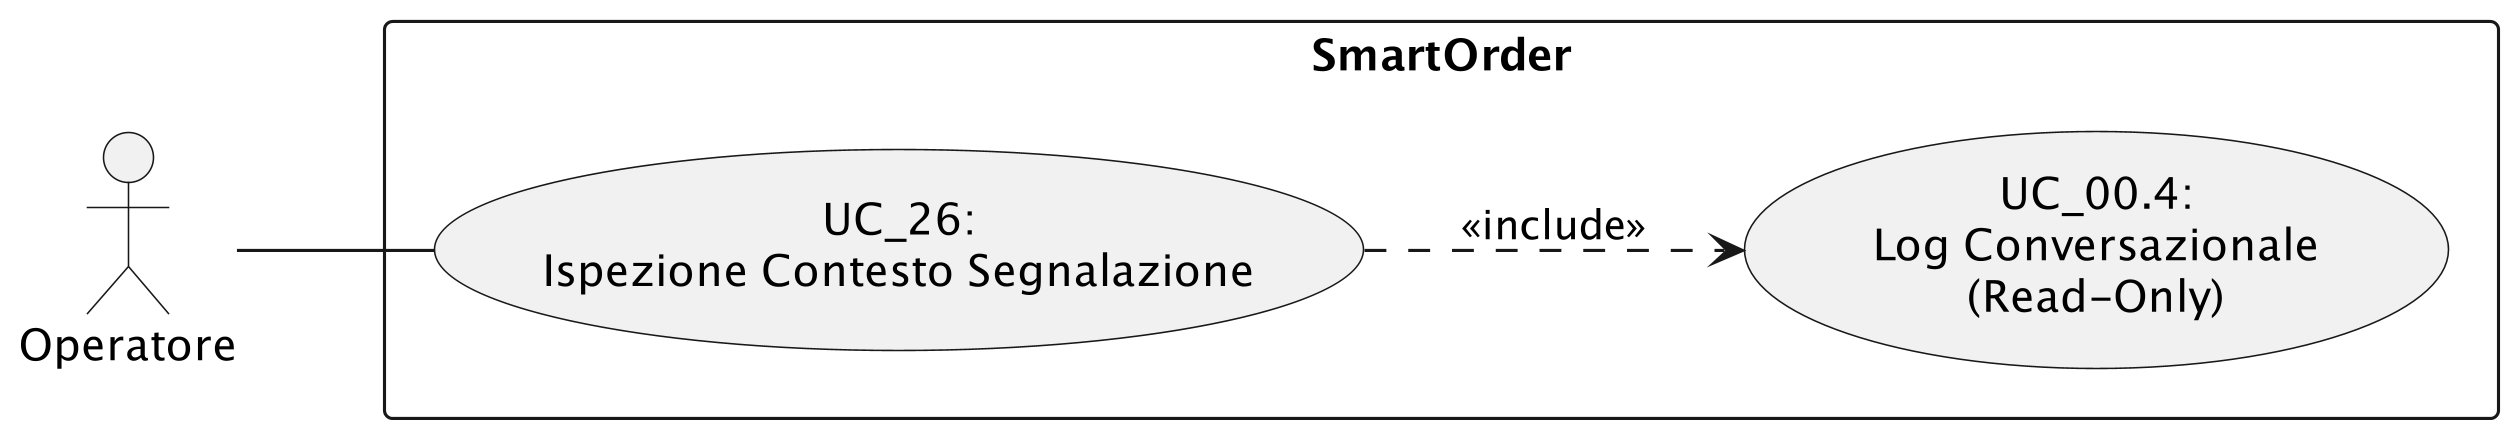
\includegraphics[width=0.7\textwidth]{uc-26.png}
    \caption{UC\_26: Ispezione Contesto Segnalazione}
\end{figure}

\begin{itemize}
    \item \textbf{Attore Principale}: Operatore
    \item \textbf{User Story}: Come Operatore, cliccando su una segnalazione in tabella, voglio poter leggere la chat originale tra il Cliente e l'AI, affinché io possa capire esattamente il contesto dell'errore prima di approvarlo o scartarlo.
    \item \textbf{Scenario Principale}: 
    \begin{enumerate}
        \item L'Operatore clicca sulla riga di una specifica segnalazione nella dashboard (\hyperref[uc_25]{UC\_25}).
        \item Il sistema istanzia una finestra di dettaglio in sovraimpressione (Modale).
        \item Il sistema recupera e mostra il tracciato storico di comunicazione (log conversazionale) associato a quella sessione $\rightarrow$ Include: \hyperref[uc_00.4]{UC\_00.4}.
    \end{enumerate}
    \item \textbf{Precondizioni}: L'Operatore sta visualizzando la tabella dell'Ottimizzazione AI e interagisce con un record valido.
    \item \textbf{Postcondizioni}: L'interfaccia espone il contesto conversazionale in modalità di sola lettura (Read-Only). L'Operatore può chiudere la modale in qualsiasi momento per tornare alla tabella.
    \item \textbf{Inclusioni}: \hyperref[uc_00.4]{UC\_00.4}
    \item \textbf{Trigger}: Click dell'Operatore su una singola segnalazione per aprirne il dettaglio.
\end{itemize}

% -------------------------------------------------------------------

\subsection{UC\_27: Validazione Segnalazione ("Da Gestire")}
\label{uc_27}

\begin{figure}[H]
    \centering 
    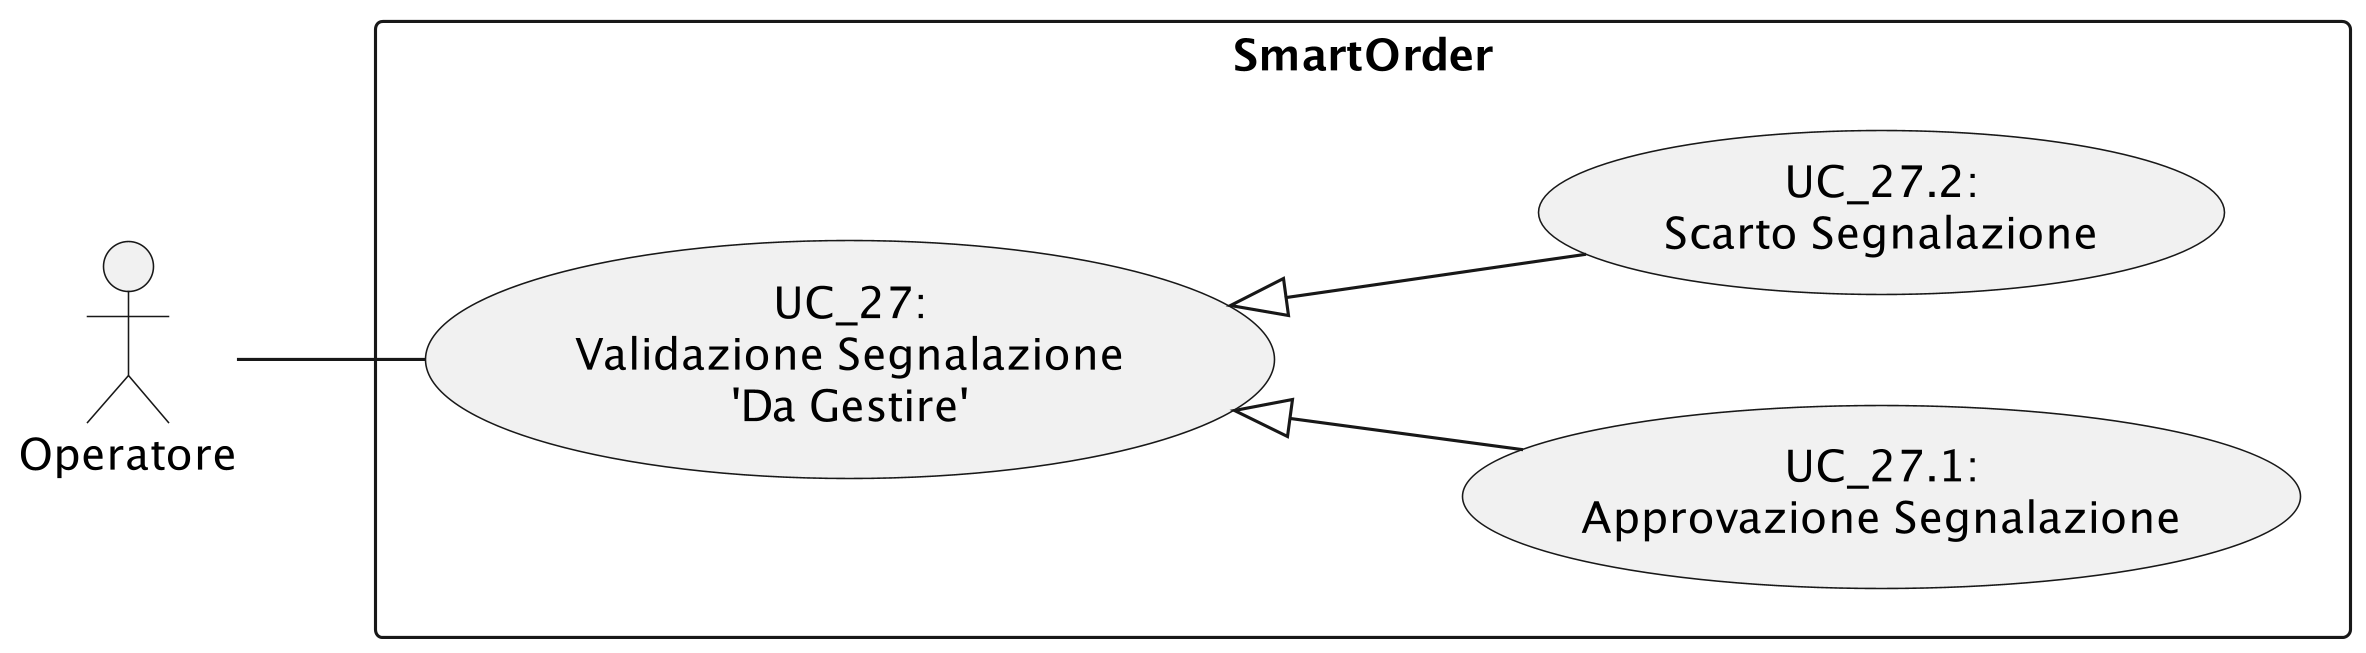
\includegraphics[width=0.7\textwidth]{uc-27.png} % Immagine del diagramma con la Generalizzazione
    \caption{Diagramma dei Casi d'Uso: Generalizzazione della Validazione}
\end{figure}

\begin{itemize}
    \item \textbf{Attore Principale}: Operatore
    \item \textbf{User Story}: Come Operatore, voglio poter definire l'esito di un'anomalia AI valutando se essa rappresenti effettivamente un errore algoritmico utile all'addestramento (Approvazione) o un falso allarme (Scarto).
    \item \textbf{Nota Architetturale}: Questo Caso d'Uso rappresenta un'astrazione generica (Validazione) che si specializza, tramite relazione di generalizzazione in UML, in due flussi operativi alternativi e mutualmente esclusivi (\hyperref[uc_27.1]{UC\_27.1} e \hyperref[uc_27.2]{UC\_27.2}).
    \item \textbf{Precondizioni}: Il record della segnalazione si trova nello stato iniziale "Da gestire".
    \item \textbf{Trigger}: Decisione dell'Operatore di prendere in carico e valutare una segnalazione pendente.
\end{itemize}

\subsubsection{UC\_27.1: Approvazione Segnalazione}
\label{uc_27.1}
\begin{itemize}
    \item \textbf{Scenario Principale}: L'Operatore innesca il comando di validazione positiva (es. pulsante "Approva") sulla riga di competenza.
    \item \textbf{Postcondizioni}: Il sistema aggiorna lo stato del record in "Accettata". I dati associati (Input utente e correzione manuale) vengono salvati e rilasciati al dataset dell'Intelligenza Artificiale per l'apprendimento continuo (Retraining).
\end{itemize}

\subsubsection{UC\_27.2: Scarto Segnalazione}
\label{uc_27.2}
\begin{itemize}
    \item \textbf{Scenario Principale}: L'Operatore innesca il comando di scarto (es. pulsante "Rifiuta"), giudicando la segnalazione come un falso positivo o un errore non imputabile all'AI.
    \item \textbf{Postcondizioni}: Il sistema aggiorna lo stato del record in "Rifiutata". I dati vengono scartati e non verranno utilizzati in alcuna operazione di Retraining.
\end{itemize}

% -------------------------------------------------------------------

\subsection{UC\_28: Revoca Segnalazione "Accettata"}
\label{uc_28}

\begin{figure}[H]
    \centering 
    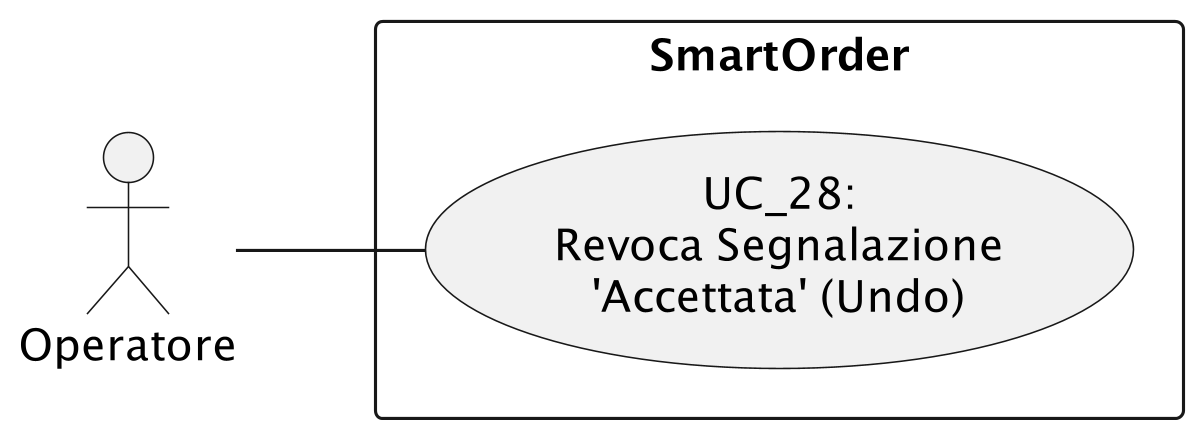
\includegraphics[width=0.6\textwidth]{uc-28.png}
    \caption{UC\_28: Revoca Segnalazione "Accettata"}
\end{figure}

\begin{itemize}
    \item \textbf{Attore Principale}: Operatore
    \item \textbf{User Story}: Come Operatore, voglio poter annullare una validazione positiva data per errore, per evitare che dati sbagliati vadano a corrompere il modello di addestramento dell'AI.
    \item \textbf{Scenario Principale}: 
    \begin{enumerate}
        \item L'Operatore filtra la tabella (\hyperref[uc_25]{UC\_25}) per visualizzare le segnalazioni già "Accettate".
        \item L'Operatore innesca il comando di ripristino (es. pulsante "Annulla/Revoca") sul record desiderato.
        \item Il sistema rimuove i dati della segnalazione dal repository di Retraining e ripristina lo stato del record a "Da gestire".
    \end{enumerate}
    \item \textbf{Precondizioni}: La dashboard espone record in stato "Accettata".
    \item \textbf{Postcondizioni}: I dati vengono invalidati ai fini dell'apprendimento e il record torna in coda per poter ricevere una nuova valutazione.
    \item \textbf{Trigger}: Click sul comando di revoca/annullamento (Undo).
\end{itemize}